\chapter{cgNA$+$ parameter sets for double-stranded nucleic acids}\label{c4}

This chapter extends the cgDNA$+$ model introduced in A. Patelli's thesis~\cite{patelithesis} to the cgNA$+$ model by estimating parameter sets for various other double-stranded nucleic acids (dsNAs).
cgNA$+$ is a coarse-grained model of dsNA (including dsDNA, dsRNA, and DNA:RNA hybrid) to predict the probability distribution function (pdf) of an arbitrary dsNA sequence (in standard A, T, C, G, U alphabets) at pre-specified physical solvent conditions.
cgNA$+$ model explicitly considers phosphates and bases as rigid bodies in $\in SE(3)$ and uses modified CURVES$+$~\cite{curveplus} helicoidal coordinates for their configuration (see \cref{c2:sec2}).
The model is trained on extensive molecular dynamics (MD) time-series (refer \cref{c2,c3}) of a comprehensive set of rationally designed sequences.
Given a sequence $\sq$ along the reading strand and a parameter set $\mathcal{P_{\text{NA}}}$ (i.e., different parameter sets are trained for different kind of dsNAs), the cgNA$+$ model predicts a Gaussian pdf in the configuration space by reconstructing a ground-state $\hat{w} (\sq, \mathcal{P_{\text{NA}}}) \in \R^{24N-18}$, and a positive-definite stiffness matrix $\K (\sq, \mathcal{P_{\text{NA}}}) \in \R^{24N-18 \times 24N-18}$:
\begin{equation}
\rho(w; \sq, \mathcal{P_{\text{NA}}}) = \frac{1}{\textit{Z}} exp \{-\frac{1}{2}(w-\hat{w})\cdot \K (w-\hat{w})\},
\label{c4:eq1}
\end{equation} 
where $\mathcal{P}_{\text{NA}}$ is the parameter set and is discussed in detail in \cref{c4:s2}.
A summary of the cgDNA$+$ model and its training procedure is in \cref{c2} and more details  can be found in ref.~\cite{patelithesis}.

In the cgNA$+$ model, we have made a few modifications in the parameter set estimation techniques from the original cgDNA$+$ model to simplify the training procedure as discussed in \cref{c4:s1} and updated the training library used to train end-block dsDNA parameters, which allows prediction of sequences with any ends (previously not possible in the cgDNA$+$ model).
Moreover, we have significantly enhanced the quality of the parameter set in the cgNA$+$ model using more extensive MD training data.
In the following \cref{c4:s2}, we have introduced the cgNA$+$ model, and in \cref{c4:s3}, we have assessed the accuracy of the model and discussed various sources of errors in the model and their quantification.
The last part presents the model's applications.
Finally, we recall that all of the discussion in this work is pertinent to dsNAs. 

Details of all the codes and data used in this chapter are provided \cref{app6}. \clearpage

\section{Updates in the cgNA$+$ model}\label{c4:s1}
The modeling aspects, including coarse-graining, various modeling assumptions, and parameter estimation in the cgNA$+$ model, remain the same as in the prior cgDNA$+$ model.
However, extending the model parameter sets for various dsNAs is a non-trivial task.
In the section, we have described the various updates or changes made in the parameter estimation procedure, MD protocol, and the training library.
These updates in the MD protocol and the training data have significantly enhanced the quality of the cgNA$+$ parameter sets.

\subsection{Modifications in parameter set estimation techniques}
The parameter set estimation procedure remains similar to that used for training the cgDNA$+$ model, except for a few changes.
In particular, in the cgDNA$+$ model, first, from the Gaussian pdf observed in the MD simulations (after filtering snapshots with broken H-bond), a banded Gaussian pdf was computed.
Then, the best-fit parameter set is estimated by minimizing the sum of KL divergences between the model reconstructions and banded Gaussian pdfs in the MD simulations for all training sequences.
In the cgNA$+$ model, the best-fit parameter set is directly computed from the observed Gaussian pdf in the MD simulations without computing the banded Gaussian pdfs.
This step simplifies the training procedure.

Moreover, estimating the parameters for various dsNAs requires several adaptations in the parameter estimation step, for example, expansion of the parameter set for DNA:RNA hybrid (DRH) as there is no Crick-Watson (CW) symmetry or the parameter set for epigenetically modified DNA requires additional (to standard) parameter blocks for modified steps.
More details are provided in \cref{c2:s4:sb3,c4:s2,c6:epi_param}.

\subsection{Updates in the MD protocol}
%The main change from the original cgDNA$+$ model is the MD protocol.
In the cgNA$+$ model, we have different parameter sets for various dsNAs trained on the extensive MD simulations of the corresponding dsNAs. 
The MD protocol to simulate training data for the cgNA$+$ model is described in \cref{c3:s2}.
As required, we have used different MD force-fields to simulate different dsNAs.
However, we have made some changes to the other MD simulation parameters. 
In particular, we have replaced the water and ion model from SPC/E~\cite{spce} and Dang ions parameters~\cite{dang1995mechanism} to TIP3P~\cite{tip3p} and Joung and Cheatham ions models~\cite{jcion}, respectively.
The previous choice of MD protocol in the cgDNA$+$ model was inspired by the MD simulations protocol used by the Ascona B-DNA Consortium~\cite{pasi2014muabc}.
However, using Dang ions parameters is no longer recommended in the Amber user manual~\cite{ambermanual}.
Therefore, we decided to change the ions parameters and move to a widely used water model, TIP3P. 
These updated choices are used for all dsNAs. 

More importantly, we have also extended the duration of MD simulations from 3 $\mu$s (used to train the cgDNA$+$ model) to 10 $\mu$s for each training sequence, which reduces the MD convergence error in terms of symmetric KL divergence and Mahalanobis distance by a factor of approximately 3.2 and 1.9 (details in \cref{c3:tab_con_dna}).

\subsection{Expansion of the training library for end-blocks parameters}
One particular limitation of the cgDNA$+$ model is that for some non-GC ends, the reconstructed/predicted stiffness matrix was non-positive definite.
As discussed earlier in \cref{c3:s3}, non-GC ends parameters in the cgDNA$+$ model are trained on a library of 15 sequences with one non-GC end followed by a random sequence, while the other end of that sequence is GC.
It implies that in the training library for end parameters, each non-GC end is followed by a particular kind of dimer step, unlike for GC ends and interior dimer steps, where all possible flanking contexts are present in the training sequences of \Lbdna.
%\rs{Qualitative explanation why the stiffness matrix is non-positive definite if the dimer is missing in the library. Is the system underdetermined?}
To better understand the kind of sequences that lead to positive-definite or non-positive definite reconstruction, we rigorously analyzed all sequences of lengths 3 to 12 and observed that GC ends always lead to a positive-definite reconstruction of the stiffness matrix, in contrast, the non-positive definite reconstructions appear only when non-GC ends are followed by a dimer that is absent in the training library.
Moreover, we observed that only one dimer case is sufficient for a positive-definite reconstruction of all the steps in that Y/R alphabets.
For example, if a training sequence is present for a non-GC end followed by AG, then the reconstructions for all sequences containing that non-GC end followed by any of the \{AG, AA, GA, GG\} are positive definite.
It suggests that the lack of diversity in the training sequences might be a possible reason for non-positive definite reconstructions. 
Even though we do not have a pure mathematical rationale, we decided to expand the training library for non-GC ends parameters empirically. 
The extended end library, \Lbe \ is provided in \cref{endlib} in which for each non-GC end, we have four training sequences such that the four sequences have one non-GC end followed by one random example dimer from each YR, RR, YY, and RY step.
In this way, we enriched the training library for non-GC ends. 
We found that using this comprehensive library, we could obtain the parameter set that guarantees positive definite reconstructions for all sequences of any length ($\geq$ 3).

\section{From cgDNA$+$ to cgNA$+$ parameter sets}\label{c4:s2}
% \subsection{Motivation for cgNA$+$}
% cgDNA/cgDNA$+$ model has been successfully implemented to explore the role of sequence-dependent DNA mechanics in persistence lengths~\cite{cgdnamc}, DNA unwrapping pathways from nucleosome core particle~\cite{pollack-cgDNA}, crystal structure packing forces~\cite{patelithesis}, and the role of histone tails in nucleosome stability~\cite{bendandi2020role}.
% Furthermore, the cgDNA$+$ model has recently been applied to scan entire genomes searching for mechanically exceptional sequences~\cite{zwahlenthesis} and obtain sequence-dependent equilibrium shapes of DNA minicircles~\cite{glowackithesis,beaud2021using}.
% Other exciting applications of the cgDNA$+$ model actively pursued in LCVMM or with collaborators include the response of DNA to external loading and twisting, computation of nucleosome wrapping energy, and prediction of protein-DNA binding affinity.
% Thus, with the overarching goal of understanding the role of DNA mechanics in its functioning in biology, the cgDNA family of models has demonstrated great potential.

% In addition to DNA as the primary genetic carrier in most organisms, RNA also carries genetic information in many viruses, besides its diverse role in biology, such as reaction catalysis, genetic information processing, and gene regulation~\cite{mandal2004gene,fire1998potent}, and is emerging as a potential therapeutic agent in clinical applications~\cite{sullenger2002emerging}.
% More details on RNA function in biology can be found in ref.~\cite{vsponer2006computational}.
% Although RNA is often present in single-stranded form, double-stranded RNA plays a prominent role in gene regulation through RNA interference (sequence-specific gene suppression)~\cite{fire1998potent}, an essential component of several tertiary structures such as riboswitches~\cite{mandal2004gene}, hairpins, and transfer RNA and forms the genome of some viruses.
% Moreover, in many biological processes~\cite{adams2012biochemistry,vella1994molecular,rich1960hybrid,brambati2020dark,meselson1958replication,shaw2008recognition}, unique heterogeneous nucleic acids are formed with one strand DNA and other strand RNA known as the DNA:RNA hybrid (abbreviated as DRH in this thesis).
% For instance, during reverse transcription, RNA viruses create transient DRH whose stability is pivotal in their replication cycle~\cite{vella1994molecular,brambati2020dark}.
% Furthermore, DRHs are seen as potential medicinal agents for conditions caused by HIV and other retroviruses~\cite{tisdale1991mutations,shaw2008recognition}. 
% One can also find a detailed account of DRH's structure and its role in biology in ref.~\cite{shaw2008recognition}.
% One particular exciting case of the role of nucleic acid mechanics in biology is RNAase H enzyme (crucial for genome stability and DNA replication of the mitochondrial genome~\cite{brambati2020dark,shaw2008recognition}) activity that can selectively recognize DRH among other double-stranded NAs (such as dsDNA and dsRNA) and degrade the RNA strand without affecting the complementary DNA strand~\cite{stein1969enzyme}, and its specificity is often attributed to various sequence-dependent structural, and mechanical features~\cite{noy2005structure,suresh2014dna,noy2008theoretical}. 
% Moreover, several experimental~\cite{zimmerman1981rna,roberts1992stability,gao1994sequence,lane1993nmr,fedoroff1997solution,szyperski1999nmr} and simulation~\cite{noy2004relative,marin2020double,noy2005structure,cheatham1997molecular,noy2005structure,suresh2014dna,priyakumar2008atomic,liu2019structural,sanghani1994theoretical,vsponer2006computational} studies revealed contrasting structural and mechanical properties of DNA, RNA, and DRH and implications in their biological functioning.

% However, these studies are performed on a limited set of sequences. 
% Therefore, a coarse-grained model such as cgDNA$+$, which predicts accurate non-local sequence-dependent mechanics of DNA, is desirable for RNA and DRH to better understand the mechanics of RNA and DRH and their role in biology.
% Thus, in this work, we have extended the cgDNA$+$ model to the cgNA$+$ model, which predicts the groundstate and stiffness of any (DNA, RNA, and DRH) sequence provided a corresponding parameter set $\mathcal{P_{\text{NA}}}$.

\subsection{cgNA$+$ parameter sets}\label{c4:subsec_prm}
cgNA$+$ is a coarse-grained model for dsDNA, dsRNA, and DRH that allows computing sequence-dependent Gaussian pdfs for an arbitrary sequence at pre-specified solvent conditions.
cgNA$+$ model is developed over the cgDNA$+$ model by estimating analogous parameters for dsRNA and DRH and improving the original cgDNA$+$ parameter set for dsDNA (updating MD protocol, more extensive and diverse training data, and simpler parameter estimation procedure) as described in the previous section.
To train the interior and GC end blocks of the cgNA$+$ parameter sets for dsDNA, dsRNA, and DRH, we have used identical training sequences (referred to as palindromic library~\cite{patelithesis}) listed in \cref{palinold}, and the same MD protocol except for force-fields to describe dsNAs.
More details on training sequences, MD protocol, and rigorous analysis of MD data are provided in \cref{c3}. 

Thus, using analogous MD time-series data for three kinds of dsNAs and parameter estimation protocol described in \cref{c2}, we have obtained three different parameter sets (one for each dsNAs), which can be written as:
\begin{equation}
\mathcal{P}_{\text{DNA}} = \{ \sigma^{5^\prime\XY},  \sigma^{\XY}, \K^{5^\prime\XY}, \K^{\XY} \} = [\R^{36}]^{16} \times [\R^{42}]^{10} \times [\R^{36 \times 36}]^{16} \times [\R^{42 \times 42}]^{10}
\label{c4:eq2_DNA}
\end{equation}
where $5^\prime\XY \in\{16$ end dimer steps$\}$  and
$\XY \in\{10$ independent dimer steps$\}$,
\begin{equation}
\mathcal{P}_{\text{RNA}} = \{ \sigma^{5^\prime\XY},  \sigma^{\XY}, \K^{5^\prime\XY}, \K^{\XY} \}  = [\R^{36}]^{1} \times [\R^{42}]^{10} \times [\R^{36 \times 36}]^{1} \times [\R^{42 \times 42}]^{10}
\label{c4:eq2_RNA}
\end{equation}
where $5^\prime\XY \in\{$GC step$\}$  and
$\XY \in\{10$ independent dimer steps$\}$, 
\begin{equation}
\begin{split}
\mathcal{P}_{\text{DRH}} & =  \{ \sigma^{5^\prime\XY},  \sigma^{\XY}, \sigma^{3^\prime\XY}, \K^{5^\prime\XY}, \K^{\XY}, \K^{3^\prime\XY} \}  \\ 
 & =  [\R^{36}]^{1} \times [\R^{42}]^{16} \times [\R^{36}]^{1} \times [\R^{36 \times 36}]^{1} \times [\R^{42 \times 42}]^{16} \times [\R^{36 \times 36}]^{1}
\end{split}
\label{c4:eq2_DRH}
\end{equation}
where $5^\prime\XY \and 3^\prime\XY \in\{$GC step$\}$  and
$\XY \in\{16$ independent dimer steps$\}$. 
The parameter for $3^\prime$ ends, and dependent dimer steps in $\mathcal{P}_{\text{DNA/RNA}}$ can be obtained using CW symmetry.
Furthermore, it must be noted that there is no CW symmetry in DRH, as reading the sequence from the DNA strand (in DRH) is chemically different from reading the sequence from the RNA strand; therefore, different parameter blocks are required for all dimers,  3$^\prime-$GC end and 5$^\prime-$GC end.
To avoid confusion in the writing and code implementation, we have always chosen the DNA strand (in DRH) as the reading strand, and the sequence is written in A/T/C/G alphabets.

\section{cgNA$+$ reconstructions and associated modeling errors}\label{c4:s3}
As mentioned earlier, the cgNA$+$ model predicts the non-local sequence-dependent groundstate of any dsDNA, dsRNA, and DRH sequence.
In this section, we have assessed the accuracy of the cgNA$+$ model by plotting the predicted groundstate for a given sequence along with the average shape obtained from the MD simulations and then quantifying the modeling error in terms of KL divergence and Mahalanobis distance.
Moreover, we have also quantified the contributions of various modeling assumptions in the total modeling error (described in \cref{c2:s3_assump}).
\subsection{Test library}
To demonstrate the generalizability of the cgNA$+$ model for any sequence, we have tested the model for a diverse set of sequences (listed in \cref{palinold}) not present in the training library. 
The test sequences contain random palindromes, A-tracts, sequences with single-nucleotide polymorphism (SNP), poly(A), poly(AT), typical \cpg islands, and long random sequences of length double that of those in the training library.
Note that some of the sequences in the test library, such as A-tracts (intrinsically bent fragments), poly-A (stiffest in terms of persistence length), and \cpg islands are mechanically exceptional sequences, and the model is not directly trained on such sequences.
For instance, sequence indices 22 and 23 in \Lbdna \ are two A-tracts of class $\text{(XA}_4\text{T}_4\text{Y)}_n$ and $\text{(XT}_4\text{A}_4\text{Y)}_n$ where X,Y $\in$ \{G, C\} which are similar in chemical composition but show contrasting differences in their super-helical structure.
To compare the cgNA$+$ model predictions with the MD estimates for the test sequences, we have generated the same length of MD time-series using the same protocol for each sequence.
Lastly, we only have an extensive test library for dsDNA and dsRNA sequences, while test sequences are limited for DRH, a choice to optimize resources.
%For example, we have included two A-tracts (sequence indices 22 and 23 in \Lbdna),  and~\cite{hognon2019cooperative} \rs{fill in details}. 
% "whose methylation status has been largely described while its aberration is correlated to cancer development affecting different organs and including breast, lungs, and the digestive tract" (the line is copy-pasted from the following article).~\cite{Cooperative effects of cytosine methylation on DNA structure and dynamics} and a few more citations in this paper
%-- A-tracts are of special interest --~\cite{drvsata2014mechanical,sprous1999molecular}
%--  A-tracts are more rigid than the control G/C-rich sequence in localized distortions relevant for nucleosome formation but are more flexible in global bending and twisting relevant for looping. \rs{compare in terms of persistence length} ~\cite{drvsata2014mechanical} \\
\subsection{Reconstruction or prediction error in cgNA$+$}
In this subsection, we first plotted the groundstate for a few selected sequences along with the observed MD estimates to visualize the accuracy of the cgNA+ model.
In \cref{c4:figure1}(a), we have plotted the groundstate ($w$) for the sequence indices 20 and 21 of \Lbdna \ (see \cref{palinold}). 
Sequence index 20 is carefully chosen to contain all independent dimer steps, while sequence index 21 is the point mutation (SNP) of the same sequence.
Moreover, along with cgNA$+$ predicted groundstate (in dashed line), we plotted the corresponding average shape from the MD time-series (in solid line).
The following observations can be made from \cref{c4:figure1}(a)
i) the cgNA$+$ model predicts the groundstate almost indistinguishable from the corresponding MD statistics. 
Remarkably, the examples provided here are not in the training sequences used to obtain cgNA$+$ model parameters;
ii) The two sequences differ by only a point mutation at the middle position; however, the change in groundstate due to that point mutation is highly non-local, i.e., up to three to four base-pairs on both sides of the mutation. 
More importantly, the cgNA$+$ model accurately captures this non-local sequence dependence in the groundstate while only using dimer-dependent parameters. 
This feature is only possible in a rigid-base model (cgDNA) or finer models (cgNA$+$) for which individual base-pair steps cannot achieve their local minima simultaneously, and frustration arises between the nearest-neighbors; thus, naturally capturing the non-local sequence-dependence in the mechanics of dsDNA but only using dimer dependent parameters~\cite{cgDNA1,petkevivciute2014cgdna,patelithesis}.

Furthermore, in \cref{c4:figure1}(b), we have plotted the predicted groundstate of two A-tracts (sequence indices 22 and 23 in \Lbdna) along with the corresponding MD average shape.
Note that the A-tracts are intrinsically bent fragments and the two A-tracts shown here have distinct super-helical structures.
%\rs{put 3D image from somewhere and cite}
It can be observed in the figure that the cgNA$+$ model accurately captures the groundstate for such mechanically exceptional sequences.
However, it is worth noting that the predictions for both sequences are not equally accurate.
For example, the predicted Propeller for sequence index 22 is equal to the value observed in MD; in contrast, for sequence index 23, the prediction for Propeller deviates from the MD observations at the TA step.
It is challenging to understand its reason precisely, and we have left a more detailed investigation for future studies.
Moreover, in \cref{c4:figure1_rna}(a), we have compared poly(A) and poly(AU) embedded in the GC ends, which are sequence indices 18 and 19 in \Lbrna \ and shown that for dsRNA sequences, cgNA$+$ model predictions are highly accurate.
Lastly, in \cref{c4:figure1_rna}(b), we have highlighted the influence of beyond tetramer context by plotting the groundstate of two dimer steps in two different beyond tetramer flanking contexts along with the corresponding MD estimates and shown that the cgNA$+$ model accurately captures such strongly non-local changes in the groundstate.

In \cref{c4:figure1,c4:figure1_rna}, we have demonstrated that the cgNA$+$ model predicts the groundstate for any dsDNA/dsRNA/DRH sequence with negligible error and is visually almost indistinguishable from the corresponding MD estimates.
Now, to quantify this error, we have defined the reconstruction or prediction error, $\er^{\text{res}}$ as the deviation of the predicted Gaussian pdf from the corresponding observed Gaussian pdf in MD simulations.
We have computed this reconstruction error in terms of symmetric KL divergence and symmetric Mahalanobis distance as defined in \cref{c2:s5sb3}. 
Note that $\er_{\text{KL}}^{\text{res}}$ (reconstruction error in terms of KL divergence) describes the total reconstruction error in the predicted groundstate and stiffness matrix while $\er_{\M}^{\text{res}}$ (reconstruction error in terms of Mahalanobis distance) highlights the difference in the predicted groundstate and MD average shape scaled by the stiffness.
In \cref{c4:tab1_errors}, we have tabulated the reconstruction errors per degree of freedom, dof (which is $24N-18$, i.e., the number of internal coordinates required to describe a given sequence of length $N$ bp) in the training and test sequences for \Lbdna, \Lbrna, and \Lbdrh. 
Firstly, the average model reconstruction errors in \Lbdna \ training sequences are 0.0020 and 0.0313 in terms of $\er_{\M}^{\text{res}}$ and $\er_{\text{KL}}^{\text{res}}$, respectively, which are approximately one order smaller than the corresponding \textit{scale} (which quantifies variation over sequence) obtained by computing the average pair-wise difference in the training sequences.
It highlights the precision of the cgNA$+$ model in capturing the non-local sequence-dependent mechanics of dsDNA. 
Similar observations can be made for dsRNA and DRH.
The average reconstruction error in test sequences ($\er_{\M}^{\text{res}} \approx 0.0027$ and $\er_{\text{KL}}^{\text{res}} \approx 0.0316$) is slightly higher than in training sequences, as most test sequences possess exceptional mechanical behavior, and such sequences are not directly present in the training set.
Therefore, an accuracy comparable to that in the training set for such exceptional sequences is highly impressive.

Note that the \textit{scale} obtained for three types of dsNAs are in the order dsDNA $>$ DRH $>$ dsRNA, even though computed identically on similar training sequences.
It can be attributed to the larger conformational space of dsDNA compared to dsRNA~\cite{noy2004relative,noy2005structure} (refer to \cref{c3:s6}).
The Gaussian pdfs for two dsDNA sequences are farther from each other in conformational space than the identical two dsRNA sequences.
Unsurprisingly, DRH lies between dsDNA and dsRNA.
Similarly, the reconstruction errors are also in the same order, since it is easier to train a model (with a fixed number of parameters) on pdfs in a smaller conformational space.

This total reconstruction error in the cgNA$+$ model results from several modeling assumptions as listed in \cref{c2:sec3} and the error associated with each assumption can be quantified as described in \cref{c2:sec5}.
We have discussed the contributions of various modeling assumptions to the reconstruction error in the following subsections.

\subsection{Approximation error in the training data}
The first modeling assumption is that the MD time-series is stationary, which is not the case. The associated convergence error (referred to as palindromic error) is discussed in \cref{c2:s5sb1}, and details on the quantification of this error are provided in \cref{c3:s5}.
For the training sequences in \Lbdna, \Lbrna, and \Lbdrh, the average palindromic errors in terms of KL divergence $\er_{\text{KL}}^{\text{palin}}$ and Mahalanobis distance $\er_{\M}^{\text{palin}}$ are of the order $10^{-4}$ and $10^{-3}$, respectively, which are approximately two orders smaller than the corresponding \textit{scales}.

Moreover, in \cref{c3:s6}, we have shown that the distributions for inter base-pair step and phosphate coordinates for dsDNA often deviate from Gaussian behavior (which also depend on the flanking sequence context).
In contrast, the distributions for various internal coordinates in dsRNA are almost Gaussian.
In DRH, we observed a mixed kind of behavior in the distribution of the internal coordinates.
However, for modeling purposes, we have imposed Gaussianity to the underlying distributions for internal coordinates, leading to an inevitable modeling error. 
We have quantified this modeling error, $\er_{\text{KL}}^{\text{Gauss}}$ by computing the KL divergence between the observed pdf and the best-fit Gaussian pdf to the observed pdf as described in \cref{c2:s5sb22} and quantified in \cref{c3:s7}.
Except for a Wtra1 phosphate coordinate, $\er_{\text{KL}}^{\text{Gauss}}$ is less than \textit{scale}.

It should be noted that the reconstruction error is defined as the deviation of cgNA$+$ predicted Gaussian pdf with the stationary observed Gaussian pdf in MD simulations, i.e., observed MD Gaussian pdf is the ground truth for the cgNA$+$ model.
Therefore, the palindromic and Gaussian approximation errors do not contribute to the aforementioned reconstruction error.

\begin{table}[H]
\begin{center}
\begin{small}
\begin{tabular}{ c || c c | c c | c c }
  \multicolumn{3}{c}{\; \; \; \; \; \; \; \; \; \ \Lbdna}& \multicolumn{2}{c}{\Lbrna}& \multicolumn{2}{c}{\Lbdrh} \\
\hline
  \multicolumn{7}{c}{Training sequences} \\
\hline
Index & $\er_{\M}^{\text{res}}$ & $\er_{\text{KL}}^{\text{res}}$ & $\er_{\M}^{\text{res}}$ & $\er_{\text{KL}}^{\text{res}}$ & $\er_{\M}^{\text{res}}$ & $\er_{\text{KL}}^{\text{res}}$ \\
\hline
1  & 0.0018 & 0.0240 & 0.0010 & 0.0058 & 0.0018 & 0.0239 \\
2  & 0.0025 & 0.0439 & 0.0011 & 0.0064 & 0.0019 & 0.0254 \\
3  & 0.0020 & 0.0302 & 0.0013 & 0.0070 & 0.0016 & 0.0227 \\
4  & 0.0016 & 0.0267 & 0.0011 & 0.0083 & 0.0015 & 0.0165 \\
5  & 0.0021 & 0.0289 & 0.0012 & 0.0081 & 0.0017 & 0.0226 \\
6  & 0.0025 & 0.0368 & 0.0013 & 0.0063 & 0.0017 & 0.0213 \\
7  & 0.0021 & 0.0353 & 0.0012 & 0.0070 & 0.0018 & 0.0209 \\
8  & 0.0017 & 0.0266 & 0.0011 & 0.0071 & 0.0015 & 0.0247 \\
9  & 0.0022 & 0.0328 & 0.0013 & 0.0080 & 0.0018 & 0.0215 \\
10 & 0.0020 & 0.0276 & 0.0011 & 0.0074 & 0.0017 & 0.0209 \\
11 & 0.0020 & 0.0342 & 0.0013 & 0.0095 & 0.0015 & 0.0167 \\
12 & 0.0020 & 0.0322 & 0.0013 & 0.0067 & 0.0017 & 0.0432 \\
13 & 0.0018 & 0.0297 & 0.0014 & 0.0101 & 0.0017 & 0.0214 \\
14 & 0.0016 & 0.0282 & 0.0014 & 0.0092 & 0.0019 & 0.0218 \\
15 & 0.0023 & 0.0344 & 0.0014 & 0.0101 & 0.0027 & 0.0395 \\
16 & 0.0017 & 0.0296 & 0.0013 & 0.0076 & 0.0047 & 0.0532 \\
\hline
\textbf{Average} & 0.0020 & 0.0313 & 0.0012 & 0.0078 & 0.0019 & 0.0260 \\
\hline
 \multicolumn{7}{c}{Test sequences} \\
\hline
Index & $\er_{\M}^{\text{res}}$ & $\er_{\text{KL}}^{\text{res}}$ & $\er_{\M}^{\text{res}}$ & $\er_{\text{KL}}^{\text{res}}$ & $\er_{\M}^{\text{res}}$ & $\er_{\text{KL}}^{\text{res}}$ \\
\hline
17 & 0.0026 & 0.0357 & 0.0015 & 0.0087 & 0.0031 & 0.1032 \\
18 & 0.0037 & 0.0291 & 0.0014 & 0.0095 \\
19 & 0.0034 & 0.0483 & 0.0021 & 0.0100 \\
20 & 0.0027 & 0.0306 & 0.0018 & 0.0101 \\
21 & 0.0026 & 0.0291 & 0.0015 & 0.0070 \\
22 & 0.0022 & 0.0285 & 0.0011 & 0.0092 \\
23 & 0.0019 & 0.0283 & 0.0010 & 0.0076 \\
24 & 0.0024 & 0.0254 & 0.0016 & 0.0061 \\
25 & 0.0027 & 0.0297 & & \\
26 & 0.0016 & 0.1449 & & \\
\hline
\textbf{Average} & 0.0027 & 0.0316 & 0.0015 & 0.0085 \\
\hline
\hline
\textbf{\textit{scale}}  & 0.0245  &  0.4395 &  0.0177  &  0.2185 &  0.0209  &  0.3273 \\
\hline
\end{tabular}
\end{small}
\end{center}
\centering\caption{
Model reconstruction error in terms of KL divergence ($\er_{\text{KL}}^{\text{res}}$) and Mahalanobis distance ($\er_{\M}^{\text{res}}$) as defined in \cref{c2:s5sb3}. 
The list of sequences is provided in the \cref{palinold} where the first 16 are training sequences, and the rest are test sequences.
The \textit{scale} (which quantifies variation over sequence) is obtained by computing the average pair-wise difference between all the training sequences.
}
\label{c4:tab1_errors}
\end{table} 

\begin{figure}[H]
  \begin{subfigure}{15cm}
    \centering\includegraphics[scale=1]{images/Xpalin_compare_thesis.pdf}
    \centering\caption{ Point mutation.}
  \end{subfigure} 

  \begin{subfigure}{15cm}
    \centering\includegraphics[scale=1]{images/DNA_compare_seq_22_23.pdf} 
    \centering\caption{ Two A-tracts. }
  \end{subfigure}
\centering\caption{Groundstate coordinates (elements of $w$) for (a) sequence indices 20 (in red, blue, and green as shown in legend) and 21 (in dark red, dark blue, dark green) and (b) sequence indices 22 (in red, blue, and green as shown in legend) and 23 (in dark red, dark blue, dark green) in \Lbdna. The figure highlights the cgNA$+$ model accuracy in capturing (a) point mutation and (b) mechanically exceptional behavior of A-tracts.
MD estimates are in solid lines while dashed lines are cgNA$+$ reconstructions.}
\label{c4:figure1}
\end{figure}
%%%%%%%%%%%%%%%%%%%%%%%%%%%%%%%%%%
\begin{figure}[H]
  \begin{subfigure}{15cm}
    \centering\includegraphics[scale=1]{images/RNA_compare_seq_18_19.pdf}
    \centering\caption{poly(A) and poly(AU).}
  \end{subfigure} 

  \begin{subfigure}{15cm}
    \centering\includegraphics{./Xray_images/hex_context_effect.pdf}
    \centering\caption{Hexamer context effect on CA and TT steps}
  \end{subfigure}
\centering\caption{(a) Groundstate coordinates (elements of $w$) for sequence indices 18 (in red, blue, and green as shown in legend) and 19 (in dark red, dark blue, dark green) in \Lbrna. MD estimates are in solid lines while dashed lines are cgNA$+$ reconstructions.
(b) Internal coordinates of middle-junction dimer in different beyond tetramer context highlighting beyond tetramer flanking context influence on groundstate of the middle-junction dimer.
The $\bullet$ is MD simulations data, and $-$ is cgNA$+$ predictions, and the two data sets are indistinguishable. 
Note that beyond hexamer flanking sequence is also different but concisely denoted as \,-\,-\,-\,.
}
\label{c4:figure1_rna}
\end{figure}

With these two approximations on MD time-series, we obtain a Gaussian pdf for each of the training sequences, which are used to compute the dimer-dependent parameter set based on two assumptions: a) the nearest-neighbor interactions assumption, i.e., the total energy of any given oligomer is the sum of local junction energies, and b) the local junction energy parameters depend only on the sequence of the corresponding junction dimer.
Note that, in the updated cgNA$+$ training protocol, we directly computed the model parameters from the observed MD Gaussian pdf, unlike previously~\cite{patelithesis}, in which the parameters were obtained in two steps, first, a banded Gaussian pdf (corresponding to the assumption of nearest-neighbor interactions) was obtained for all training sequences followed by the estimation of dimer-dependent parameters.
As a consequence of this direct computation, we cannot precisely determine the error associated with these two assumptions. 
However, we can approximate the errors associated with these two assumptions a) by computing the banded stiffness matrix, which corresponds to nearest-neighbor interactions from the observed stiffness matrix in MD simulations, and then defining the truncation error as the KL divergence between banded and observed Gaussian pdfs and b) sequence locality error in the junction energy parameters by computing the KL divergence between banded and reconstructed Gaussian pdfs.

\subsection{Contribution of nearest-neighbor interactions assumption in cgNA$+$ reconstruction error}\label{c4:s3sb1}
Firstly, note that even though the nearest-neighbor interactions assumption simplifies the modeling, it is based on the observations made in the MD statistics.
In \cref{c4:fig2_stiffness}, we have plotted the observed stiffness matrix in MD time-series for sequence index 1 in \Lbdna \ along with the stencils corresponding to the nearest-neighbor interactions approximation. 
Note that the stiffness matrix is shown for only half of the sequence as the remaining entries are dependent due to the palindromic nature of the sequence. 
It can be observed from the plot that the stiffness matrix is highly banded, and there are very few entries outside the stencils, thus, justifying the nearest-neighbor interactions approximation.
However, it must be noted that the non-zero entries outside the stencils are located very close to the stencils, which may suggest developing a model beyond nearest-neighbor interactions.
The possibility of next-to-nearest-neighbor interactions is discussed in refs.~\cite{patelithesis,cgDNA1,petkevivciute2014cgdna}.
These works concluded that extending the current nearest-neighbor to next-to-nearest-neighbor interactions approximation would lead to a significant increase in model parameters, while the gain in accuracy will be comparatively smaller.
Moreover, with more model parameters, training the model and ensuring a positive-definite reconstruction for any sequence will be challenging.
Therefore, in the cgNA$+$ model, we continued with the nearest-neighbor interactions approximation.
We want to emphasize that the accuracy gained in the model from cgDNA to cgDNA$+$ is remarkable, as discussed in ref.~\cite{patelithesis}.
Moreover, we found a similar sparsity pattern in the observed MD stiffness matrix for dsRNA and DRH as shown in \cref{c4:fig3_stiffness} for sequence index 1 in \Lbrna \ and \Lbdrh. 
Note that the sequence in \Lbdrh \ is not palindrome, but we plotted half stiffness matrix for better visualization and comparison.

To quantify the error associated with this approximation, we have first computed the banded stiffness matrix corresponding to the nearest-neighbor interactions approximation using the maximum entropy fit algorithm~\cite{glowackithesis}.
Then this approximation error (referred to as truncation error, $\er_{\text{KL}}^{\text{Trunc}}$) can be computed as the symmetric KL divergence between the observed stiffness and the corresponding banded stiffness as given in \cref{c2:s5sb3}.
Note that the corresponding Mahalanobis contribution will be zero, since there is no change in the average shape of the oligomer when computing the banded stiffness (refer \cref{a3:eq12}). In \cref{c4:tab3_errors}, we have listed the truncation errors, $\er_{\text{KL}}^{\text{Trunc}}$ for the training sequences (for brevity, we have not provided results for all sequences) in \Lbdna, \Lbrna, and \Lbdrh.
It can be observed that for all sequences $\er_{\text{KL}}^{\text{Trunc}}$ is almost similar, with average values of 0.0046, 0.0026, and 0.0049 per dof for dsDNA, dsRNA, and DRH, respectively, which is approximately 100 times smaller than the corresponding \textit{scale}.

Lastly, the truncation error in dsRNA sequences is approximately half of the error in dsDNA sequences, which might be attributed to the larger conformational space of dsDNA/DRH, but can not be ascertained.

\subsection{Contribution of sequence locality assumption in cgNA$+$ reconstruction error}\label{c4:s3sb2}
The final assumption in the cgNA$+$ model is the dependence of local junction energy parameters on the local dimer sequence.
For instance, in $\mathcal{P}_{\text{DNA}}$, $\sigma^{\XY}$ and $\K^{\XY}$ depend on the local dimer step XY. 
Note that the position of a given junction is crucial; therefore, we have different parameters for the interior and terminal junctions.
The errors associated with this assumption, $\er_{\text{KL}}^{\text{local}}$ and $\er_{\M}^{\text{local}}$ (described in \cref{c2:s5sb23_local}), are tabulated in \cref{c4:tab3_errors} for training sequences in \Lbdna, \Lbrna, and \Lbdrh.
Remarkably, $\er_{\text{KL}}^{\text{local}}$ and $\er_{\M}^{\text{local}}$ are at least one order of magnitude smaller than the corresponding \textit{scale} for each training sequence in \Lbdna, \Lbrna, and \Lbdrh.

\begin{table}[H]
\begin{center}
\begin{small}
\begin{tabular}{ c || c c c | c c c | c c c}
\multicolumn{4}{c}{\; \; \; \; \; \; \; \; \; \ \Lbdna}& \multicolumn{3}{c}{\Lbrna}& \multicolumn{3}{c}{\Lbdrh} \\
\hline
Index & $\er_{\text{KL}}^{\text{Trunc}}$ & $\er_{\M}^{\text{local}}$ & $\er_{\text{KL}}^{\text{local}}$ &  $\er_{\text{KL}}^{\text{Trunc}}$ & $\er_{\M}^{\text{local}}$ & $\er_{\text{KL}}^{\text{local}}$ & $\er_{\text{KL}}^{\text{Trunc}}$ & $\er_{\M}^{\text{local}}$ & $\er_{\text{KL}}^{\text{local}}$ \\
\hline
1   & 0.0046 &  0.0018  &  0.0198  & 0.0026 &  0.0011  &  0.0034  & 0.0051 &  0.0019  &  0.0196 \\
2   & 0.0048 &  0.0026  &  0.0401  & 0.0026 &  0.0012  &  0.0039  & 0.0050 &  0.0019  &  0.0213 \\
3   & 0.0046 &  0.0021  &  0.0260  & 0.0025 &  0.0014  &  0.0047  & 0.0049 &  0.0017  &  0.0185 \\
4   & 0.0046 &  0.0016  &  0.0228  & 0.0025 &  0.0012  &  0.0060  & 0.0047 &  0.0016  &  0.0125 \\
5   & 0.0048 &  0.0021  &  0.0249  & 0.0025 &  0.0013  &  0.0058  & 0.0049 &  0.0017  &  0.0185 \\
6   & 0.0045 &  0.0026  &  0.0328  & 0.0026 &  0.0013  &  0.0039  & 0.0047 &  0.0018  &  0.0172 \\
7   & 0.0043 &  0.0022  &  0.0314  & 0.0026 &  0.0013  &  0.0046  & 0.0048 &  0.0019  &  0.0168 \\
8   & 0.0047 &  0.0017  &  0.0224  & 0.0025 &  0.0011  &  0.0047  & 0.0049 &  0.0016  &  0.0206 \\
9   & 0.0046 &  0.0022  &  0.0288  & 0.0026 &  0.0014  &  0.0057  & 0.0051 &  0.0019  &  0.0173 \\
10  & 0.0045 &  0.0021  &  0.0236  & 0.0026 &  0.0012  &  0.0051  & 0.0053 &  0.0018  &  0.0166 \\
11  & 0.0043 &  0.0021  &  0.0305  & 0.0026 &  0.0013  &  0.0071  & 0.0045 &  0.0015  &  0.0127 \\
12  & 0.0046 &  0.0021  &  0.0284  & 0.0025 &  0.0014  &  0.0044  & 0.0050 &  0.0018  &  0.0393 \\
13  & 0.0050 &  0.0018  &  0.0255  & 0.0026 &  0.0014  &  0.0077  & 0.0055 &  0.0017  &  0.0172 \\
14  & 0.0043 &  0.0017  &  0.0242  & 0.0025 &  0.0015  &  0.0069  & 0.0049 &  0.0019  &  0.0176 \\
15  & 0.0046 &  0.0023  &  0.0306  & 0.0027 &  0.0014  &  0.0077  & 0.0048 &  0.0028  &  0.0355 \\
16  & 0.0046 &  0.0017  &  0.0255  & 0.0024 &  0.0013  &  0.0053  & 0.0049 &  0.0047  &  0.0491 \\
\hline
\textbf{Average} & 0.0046 & 0.0021  &  0.0273  & 0.0026 & 0.0013  &  0.0054  & 0.0049 &  0.0020  &  0.0219 \\
\hline
\hline
\textbf{\textit{scale}}  & 0.4395 & 0.0245  &  0.4395 & 0.2185 & 0.0177  & 0.2185 & 0.3273 &  0.0209  &  0.3273 \\
\hline
\end{tabular}
\end{small}
\end{center}
\centering\caption{Truncation error due to nearest-neighbor interactions assumption in terms of symmetric KL divergence ($\er_{\text{KL}}^{\text{Trunc}}$) and locality error due to sequence locality assumption in the junction parameters in terms of KL divergence ($\er_{\text{KL}}^{\text{local}}$) and Mahalanobis distance ($\er_{\M}^{\text{local}}$). The list of sequences are provided in the \cref{palinold}. The \textit{scale} (which quantifies variation over sequence) is obtained by computing the average pair-wise difference between all the training sequences.
}
\label{c4:tab3_errors}
\end{table}\clearpage

%%%%%%%%%%%%%%%%%%%%%%%%%%%%%%%%%%%%%%%%%%%%%%%%
\begin{figure}
  \begin{subfigure}{15cm}
    \centering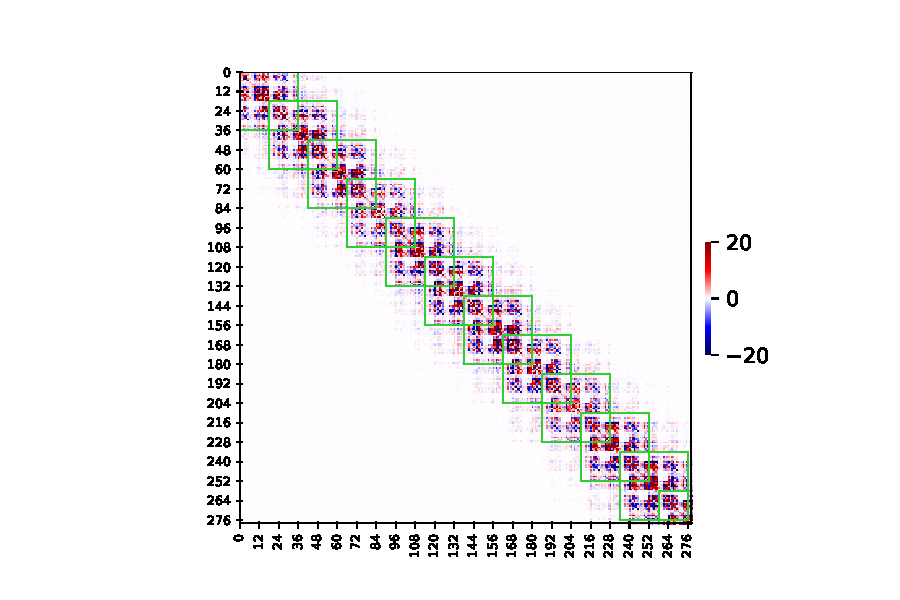
\includegraphics[trim=1cm 0.35cm 1cm 0.05cm]{images/DNA_stiffness_1.pdf}
    \centering\caption{Stiffness matrix observed in MD simulations for sequence 1 in \Lbdna}
  \end{subfigure} 

  \begin{subfigure}{15cm}
    \centering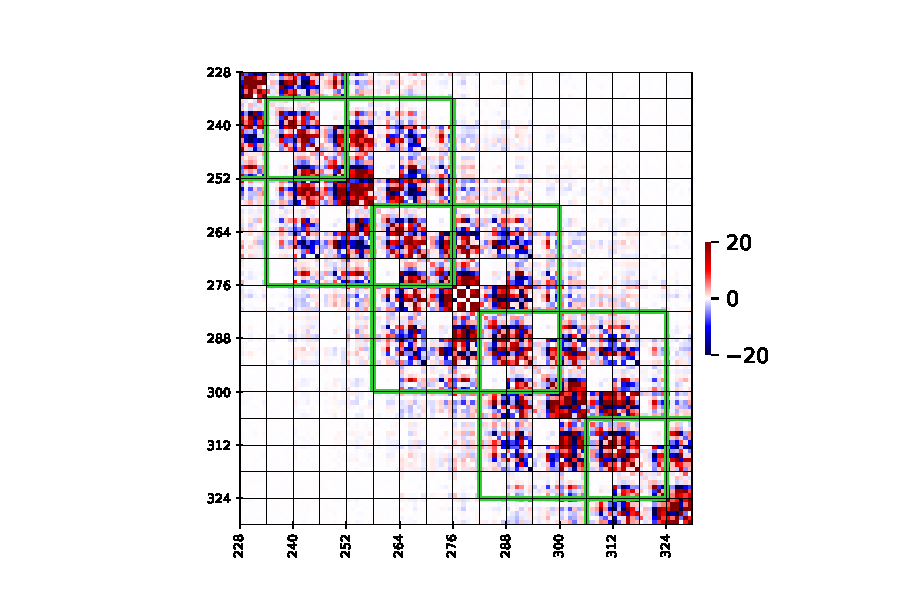
\includegraphics[trim=1cm 0.35cm 1cm 0.05cm]{images/DNA_stiffness_submatrix_1.pdf}
    \centering\caption{Enlarged version of the above plot for central tetramer}
  \end{subfigure}
\centering\caption{
(a) Sparsity pattern in observed stiffness matrix in MD simulation for sequence index 1 in \Lbdna \ (only half sequence is shown as the sequence is a palindrome), and (b) is a zoom-in image of the same matrix corresponding to central tetramer of the sequence. 
The green stencils correspond to the nearest-neighbor interactions approximation.
}
\label{c4:fig2_stiffness}
\end{figure}\clearpage
%%%%%%%%%%%%%%%%%%%%%%%%%%%%%%%%%%%%%%%%%%%%%%%%
\begin{figure}[H]
  \begin{subfigure}{15cm}
    \centering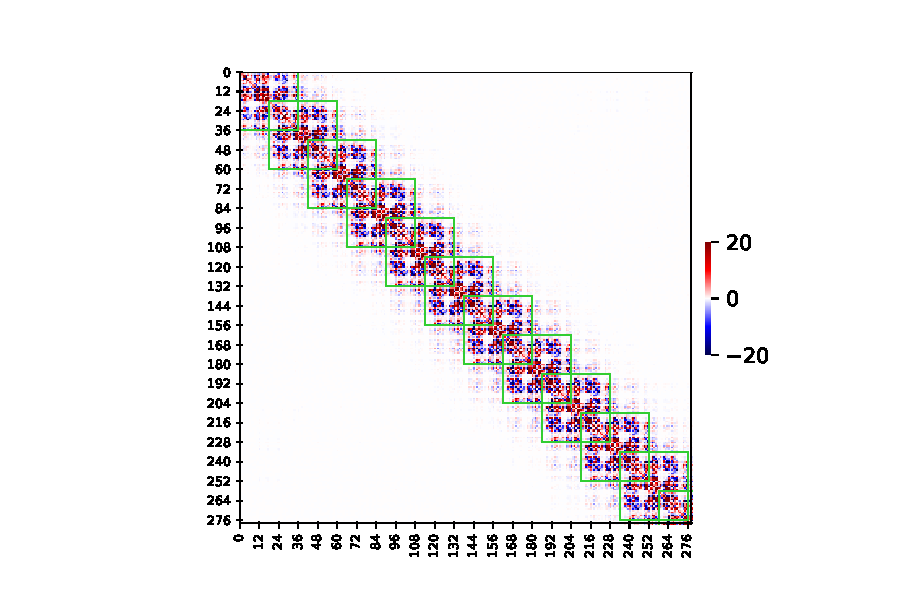
\includegraphics[trim=1cm 0.35cm 1cm 0.05cm]{images/RNA_stiffness_1.pdf}
    \centering\caption{Stiffness matrix observed in MD simulations for sequence 1 in \Lbrna}
  \end{subfigure} 

  \begin{subfigure}{15cm}
    \centering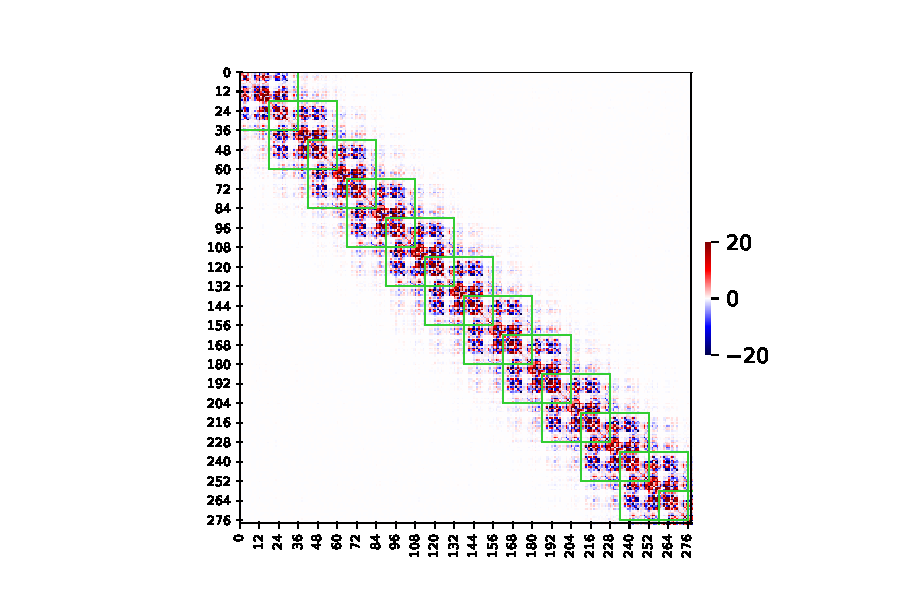
\includegraphics[trim=1cm 0.35cm 1cm 0.05cm]{images/HYB_stiffness_1.pdf}
    \centering\caption{Stiffness matrix observed in MD simulations for sequence 1 in \Lbdrh}
  \end{subfigure}
\centering\caption{
Sparsity pattern in observed stiffness matrix in MD simulation for sequence index 1 (a) in \Lbrna \ and (b) in \Lbdrh \ (only half sequence is shown). 
The green stencils correspond to the nearest-neighbor interactions approximation.
}
\label{c4:fig3_stiffness}
\end{figure}\clearpage

%%%%%%%%%%%%%%%%%%%%%%%%%%%%%%%%%%%%%%%%%%%%%%%%

Now, of these two sources ($\er^{\text{Trunc}}$ and $\er^{\text{local}}$) in the total reconstruction error ($\er^{\text{res}}$), the locality assumption in sequence dependence of local junction energy parameters dominates.
For instance, for training sequences in \Lbdna, the average reconstruction error in terms of KL divergence, $\er_{\text{KL, avg}}^{\text{res}}$ is 0.0313, of which the contribution from the nearest-neighbor interactions assumption is 0.0046 and the locality assumption in the sequence dependence of junction energy parameters is 0.0273. % 0.0273 + 0.0046 = 0.0319
This implies that the nearest-neighbor interactions assumption is reasonable and contributes negligibly to the modeling error. 
Whereas, the primary source of modeling error is the sequence locality assumption in junction energy parameters.
Once again, this error, $\er^{\text{local}}$ is only a fraction of the \textit{scale} set by computing the pair-wise difference between the training sequences in the respective libraries. 
Anyhow, it highlights the non-local sequence dependence in the local junction energy.
We would like to remind the reader that $\er_{\text{KL, avg}}^{\text{res}}$ or $\er_{\text{KL, avg}}^{\text{local}}$ has two components, Mahalanobis (which quantifies the error in the groundstate) and stiffness component (which quantifies the error in the stiffness matrix).
Further note that the Mahalanobis contribution in $\er_{\text{KL, avg}}^{\text{res}}$ or $\er_{\text{KL, avg}}^{\text{local}}$ is relatively negligible, thus implying that the major error is in the stiffness matrix, which has a dimer/trimer local sequence dependence.
Remarkably, groundstate has a highly non-local sequence dependence due to the inversion of the stiffness matrix and the corresponding frustration energy associated with it.
Lastly, we would like to recall that in the last two subsections, we have only approximated the contributions due to the nearest-neighbor interactions assumption and local sequence dependence in the junction energy parameters.
cgNA$+$ model performs the computation for these two approximations in one step, and therefore, it is impossible to quantify the associated error individually. 
Truncation using different methods may lead to slightly different quantification of these errors~\cite{petthesis,entropy}.

\section{Comparison of dsDNA, dsRNA, and DNA:RNA hybrid} \label{c4:s5}
In the previous sections, we established that the cgNA$+$ model is extremely accurate in predicting groundstate and stiffness matrix for any given dsDNA/dsRNA/DRH sequence and quantified the associated errors. 
Moreover, the prediction is extremely fast, making possible the reconstruction of groundstate and stiffness matrix for millions of sequences and, thus, statistical estimation of various dsNA properties. 
For example, one can compute groove widths for all decamers and obtain statistical conclusions about sequence-dependence in groove widths. 
Such a computation is otherwise impossible to perform using traditional computational or experimental techniques.
This section has rigorously investigated various such observables for dsDNA, dsRNA, and DRH for a large sequence space and compared the trends in these three kinds of dsNA.
Some such comparisons can be found for various dsNAs in refs.~\cite{noy2004relative,noy2005structure,marin2020double,vsponer2006computational,suresh2014dna,priyakumar2008atomic,cheatham1997molecular,perez2004relative}; however, most of these studies are done for a minimal number of sequences (often less than 5) that question the generalizability of those results, especially when it is known that the properties/features of dsNAs are highly sequence-dependent (often non-local dependence)~\cite{balaceanu2019modulation,beveridge2004molecular,dixit2005molecular,pasi2014muabc,lavery2010systematic}. \clearpage

\subsection{Comparison of average shape of dsDNA, dsRNA, and DNA:RNA hybrid} \label{c4:s5sb1}
This subsection compares the average shape of base-pairs and base-pair steps in the average flanking context for dsDNA, dsRNA, and DRH. 
Moreover, we have highlighted the sensitivity of dimer average shape to the flanking context.
For this comparison, we have used statistics obtained from MD simulations of \Lbdna, \Lbrna, and \Lbdrh \ along with the corresponding cgNA$+$ predictions (which also allowed comparing MD statistics with cgNA$+$ predictions).
We have extracted average intra base-pairs coordinates and inter base-pair step and phosphate coordinates in average flanking contexts and tetramer flanking contexts and plotted intra base-pair coordinates in \cref{c4:fig4_moncomp} and inter base-pair step and phosphate coordinates in \cref{c4:fig4_dimercomp}.

It should be noted that such comparisons have been made previously in the literature~\cite{cheatham1997molecular,noy2004relative}; however, for only limited sequences. 
Therefore, some trends in the dimer sequence dependence, particularly for inter base-pair coordinates, have been observed before; notably, this is subjected to the source of data, such as experimental X-ray data or MD simulation data using various MD protocols.
The objective of such comparison is that at length scales at which a few MD simulations can be performed, the cgNA$+$ model accurately captures the underlying trends in the average shape.

\begin{figure}[H]
\begin{center}
 \centering\includegraphics[trim=0cm 0.7cm 0cm 0cm]{images/compare_mon_gs_DNA_RNA_HYB_gs.pdf}
\end{center}
\centering\caption{
Comparison of intra base-pair coordinates for dsDNA (in Blue), dsRNA (in Red), and DRH (in Black) at the X-axis. For each base-pair in average context, coordinates observed in MD simulations and cgNA$+$ predictions are plotted in $\bullet$ and $\times$, respectively, along with the coordinates in various flanking trimer contexts in vertical lines ($|$) to highlight the role of flanking sequence.
A line plot is plotted along $\bullet$ for better visualization, and the data corresponding to dsDNA, dsRNA, and DRH is slightly shifted along the X-axis.
}
\label{c4:fig4_moncomp}
\end{figure}

This work presents the most extensive comparisons of the average shape of base-pair and base-pair steps (along with phosphate coordinates) for dsDNA, dsRNA, and DRH. In \cref{c4:fig4_moncomp,c4:fig4_dimercomp}, we have one panel for each of the internal coordinates, and the value of the given internal coordinate is plotted on the Y-axis while base-pair or base-pair step is plotted on the X-axis. 
The cgNA$+$ predictions are plotted as $\times$ in blue, red, and black for dsDNA, dsRNA, and DRH, respectively, together with the MD observations as $\bullet$.
% Moreover, for each base-pair or base-pair coordinate in the average context, we plotted the corresponding values in various trimer or tetramer flanking contexts, respectively, in vertical lines ($|$) to highlight the sensitivity to flanking contexts (observed in MD simulations).
% Moreover, we have drawn a line connecting $\bullet$, and slightly shifted the plots for dsDNA and DRH along the X-axis for better visualization and comprehension of the data. 

In \cref{c4:fig4_moncomp}, we have compared intra base-pair coordinates. 
Comparing MD observations ($\bullet$) with the corresponding cgNA$+$ predictions ($\times$), which are almost superimposed, again highlights the cgNA$+$ model accuracy.
Note that for dsDNA and dsRNA, AT and TA base-pairs and GC and CG base-pairs represent the same physical base-pair except for reading the sequence from the different strand (Watson or Crick). 
Therefore, intra base-pair coordinates for these base-pairs are the same except for the sign convention determined by the change of reading strand transformation (refer to \cref{c2:sec3sb1}).
The same is not true for DRH as the GC base-pair has G on DNA strand and C on RNA strand in contrast to the CG base-pair, which has C on DNA strand and G on RNA strand, thus representing two chemically different molecules.
Therefore, one can observe that the intra coordinates for A/T (or U) and G/C are identical (except for Buckle and Shear, in which coordinates are anti-symmetric due to reading strand transformation).
For Buckle and Shear, the average values for A and G (the independent set of base-pairs) are in the order dsDNA $>$ dsRNA $>$ DRH, with sequence average values (up to 3 decimal points) equal to 0.000 (rad/5 and \AA) for dsRNA and dsDNA and -0.456 rad/5 and -0.058 \AA \ for DRH.
Note that  the difference in magnitude is much smaller for Shear than Buckle.
Furthermore, it is interesting that in A and G, the direction of Buckle for dsDNA and DRH is opposite but with a similar magnitude.
On the contrary, for dsRNA, it remains closer to zero (planarity).
Propeller values observed in dsRNA are more negative than in dsDNA, whereas DRH adopts intermediate values of dsDNA and dsRNA.
A similar trend is also observed in Stagger with DRH values relatively closer to dsRNA.
The order is dsRNA $>$ DRH $>$ dsDNA for Opening. Lastly, for Stretch, the values for dsDNA, dsRNA, and DRH are incredibly close, with almost zero Stretch for the A-T base-pair and slightly negative Stretch for the C-G base-pair, which can be attributed to the three H-bonds in C-G as compared to two in A-T base-pair. 
Similar observations can be made for Propeller and Opening, where the average values for the C-G base-pair tend to stay close to zero, whereas, in the A-T base-pair, the deviation from zero is more. 
Lastly, from the spread of the vertical lines ($|$) around $\bullet$, it can be concluded that flanking trimer contexts significantly impact intra-base-pair coordinates with the variation due to flanking contexts often being larger than the variation for different base-pairs.
Moreover, similar trends are observed for all three dsNAs considered in this work.

Furthermore, for inter base-pair step and phosphate coordinates, out of the 16 dimers, six are dependent in the case of dsDNA and dsRNA, while for DRH, 16 dimers are independent as there is no CW symmetry. 
Therefore, \cref{c4:fig4_dimercomp} contains data corresponding to all the 16 dimers.
To start with the discussion, we focused on helical inter coordinates (Shift, Slide, Rise, Tilt, Roll, and Twist).
Shift and Tilt are odd parameters (i.e., change sign on reading strand transformation as described in \cref{c2:sec3sb1}); therefore, the average value for all dimers and palindromic dimers (AT, GC, CG, and TA) of Shift and Tilt over various dimers in the average context is zero, while the rest six dependent pairs are in positive and negative pairs. 
Shift for dsRNA remains very close to zero, while it fluctuates between positive and negative values for dsDNA.
Shift for DRH is always positive, with an average value of 0.189 \AA.
The same observations are true for Tilt, with values for dsRNA close to zero and relatively larger sequence-dependent fluctuations around zero for dsDNA.
At the same time, Tilt values for DRH are always positive with clear dimer sequence dependence.
The trends for Slide are in the order dsDNA $>$ DRH $>$ dsRNA with an average Slide of around -0.397 \AA \ for dsDNA, -1.666 \AA \ for dsRNA, and in between dsDNA and dsRNA for DRH but slightly closer to dsRNA.
The average Twist in dsDNA is considerably higher than in dsRNA due to the B-form and A-form of dsDNA and dsRNA, whereas DRH has a mixed A and B-form with A-form dominating and Twist, in general, close to dsRNA.
In particular, Noy et al.~\cite{noy2005structure} had similar findings, with Twist and Slide values being closer to the observed values in dsRNA, while the rest of the inter-coordinates are in between dsDNA and dsRNA.
%\rs{Notably for YR steps, Twist for DNA is closer to RNA, which is because A-form DNA}
It is interesting that Rise is greater for dsRNA than dsDNA for YR steps, whereas it is reversed for the rest of the dimer steps.
The Rise for DRH varies between dsDNA and dsRNA values, but is generally closer to the values observed for dsRNA.
%\rs{need to connect this with the characterization of A/B form and the coupling of Rise with Twist}
Lastly, it is evident from the spread of the vertical lines ($|$) around $\bullet$ that the tetramer context is crucial and highly influences the average shape of the dimer (in terms of inter-helical coordinates).
In particular, for inter-translational coordinates, dsDNA dimers are much more sensitive to flanking tetramer context than dsRNA, whereas DRH is in between dsDNA and dsRNA.
The trends are still very similar for rotational coordinates, but the difference is relatively smaller. 
Note that the dsDNA backbone fluctuates more and occupies a larger conformational space~\cite{noy2004relative,noy2005structure} and is coupled with inter base-pair step coordinates leading to a higher sensitivity of dsDNA inter coordinates to flanking context compared to dsRNA and DRH.

Finally, such an analysis for phosphate coordinates is entirely novel.
For DRH, we chose the DNA strand as the reading strand and the RNA strand as the complementary strand.
First, one can observe that the phosphate coordinates for dsDNA and dsRNA are very different (except WTra2 and CTra2), which can be attributed to the A- and B-form geometry of the dsNA in dsRNA and dsDNA, respectively.
Furthermore, in contrast to inter base-pair coordinates, the observed phosphate coordinates in DRH are not in between dsDNA and dsRNA; instead, Watson phosphate coordinates are closer to those observed in dsDNA, whereas Crick phosphates are closer to those observed in dsRNA.
This implies that the backbone behavior of the DNA strand in DRH is closer to pure dsDNA, and the RNA strand is closer to pure dsRNA. 
Similar findings have been reported in~\cite{noy2005structure,noy2008theoretical,cheatham1997molecular,liu2019structural} but are characterized differently.
Notably, dimer-step-dependent fluctuations in phosphate coordinates for dsDNA are considerably higher than those in dsRNA.
Moreover, for a given dimer step, the differences in average phosphate coordinates for various flanking tetramer contexts are also much higher in dsDNA than in dsRNA.
This behavior can be expected as the dsDNA backbone exhibits a larger conformational space (geometry can also change from B- to A-form depending on sequence) than dsRNA (mostly adhering to A-form geometry).
In the case of DRH, once again, it can be observed that the DRH Crick strand behaves similar to pure dsRNA (with less variation due to the dimer step sequence and the flanking tetramer context), and the Watson strand behaves similar to pure dsDNA (i.e., sensitive to dimer step sequence and flanking tetramer context). \clearpage

\subsection{Comparison of persistence lengths of dsDNA, dsRNA, and DNA:RNA hybrid}\label{c4:s5sb3}
One of the most popular and traditional measures to quantify the rigidity of the NAs is persistence length, which can be defined as the length scale over which correlations in the direction of tangent along a polymer centerline are lost~\cite{hagerman1988flexibility}. 
In the context of DNA (and other NAs), the definition of persistence length has been traditionally and frequently used in the sequence-average sense, which has two crucial governing factors, stiffness and intrinsic shape~\cite{trifonov1987dna}. 
However, it is well understood that both governing factors depend on the sequence of the given NA.
Mitchell et al.~\cite{cgdnamc} rigorously studied sequence-dependent persistence lengths of dsDNA (referred to as apparent persistence length, $\ell_{p}$) using the cgDNA model and, for the first time, introduced the notion of sequence-dependent dynamic persistence length, $\ell_{d}$ by factoring out the contributions of the intrinsic shape from $\ell_{p}$.
This work has been summarized in \cref{c2:sec6} in the context of the cgNA$+$ model, and more details can be found in refs.~\cite{patelithesis,cgdnamc}.

We want to remind the readers that persistence length is also sensitive to experimental techniques and conditions, along with sequence dependence.
For example, increasing the salt concentration decreases the persistence length of dsDNA from 57 to 43 nm. 
In the present literature, 150 bps or 50 nm is the agreed sequence-average persistence length of the dsDNA. 
The persistence length predicted by the cgDNA or cgDNA$+$ model is, in general, considerably higher than the experimental consensus of 150 bps.
It has been thoroughly discussed in previous work~\cite{patelithesis,cgdnamc} where they demonstrated that although the model predictions are higher than experimental consensus, the trends in sequence-dependent persistence lengths of dsDNA are similar to those observed in the experiments.
There can be several reasons for this discrepancy of persistence lengths given by cgNA$+$ tools.
Firstly, in experiments, the salt concentration is relatively higher, and often divalent counter ions are used as opposed to mono-valent ions under physiological concentrations in the MD simulations (used to train the cgNA$+$ model), which have a significant effect on the persistence length of dsDNA (or dsNA)~\cite{savelyev2012monovalent,zhang2019mechanical,brunet2015dependence}.
Moreover, the parameterization of DNA in various MD forcefields might be stiffer~\cite{parmbsc1,dans2017accurate}.  
Notably, it has been shown in ref.~\cite{patelithesis} that for shorter sequences (24mer), the tangent-tangent correlation observed in the MD simulations is incredibly close to cgDNA$+$ predictions implying that this discrepancy is not inherent to the model.

Such a rigorous study of the persistence lengths of dsRNA and DRH is entirely novel.
A few experimental investigations have measured the persistence length of a few dsRNA sequences in various experimental setups, again providing very different values of the persistence length for dsRNA.
However, in general, the dsRNA is considered to be stiffer than dsDNA.
Experiments~\cite{abels2005single} performed using magnetic tweezers and atomic force microscopy (believed to be highly accurate experimental techniques to measure persistence length) found that the mean persistence length of dsRNA is equal to 63.8 and 62 nm, respectively.
%This increased rigidity of RNA compared to DNA can be ascribed to RNA's A-form geometry, leading to the interference of the $2^\prime-$OH with the sugar arrangement in the backbone.
In the case of DRH, Zhang et al. ~\cite{zhang2019mechanical} found the persistence length of DRH $\approx 63$ nm at one mM NaCl.
Moreover, magnetic tweezers experiments at various salt conditions have shown that the persistence length of DRH is generally in between dsDNA and dsRNA.
Lastly, all such experiments are performed under specific conditions and for limited sequences, making it difficult to draw any statistical conclusions about the persistence length of dsNAs.\clearpage

\begin{figure}[p]
\begin{center}
 \centering\includegraphics[width=14.9cm,trim=0cm 0.7cm 0cm 0cm]{images/compare_dim_gs_DNA_RNA_HYB_gs.pdf}
\end{center}
\centering\caption{
Comparison of base-pair step and phosphate coordinates for dsDNA (in Blue), dsRNA (in Red), and DRH (in Black) at the X-axis. For each base-pair step in average context, coordinates observed in MD simulations and cgNA$+$ predictions are plotted in $\bullet$ and $\times$, respectively, along with the coordinates in various flanking tetramer contexts in vertical lines ($|$) to highlight the role of flanking sequence.
For better visualization, a line plot is plotted along $\bullet$, and the data corresponding to dsDNA, dsRNA, and DRH is slightly shifted along the X-axis.
}
\label{c4:fig4_dimercomp}
\end{figure}  
\clearpage




In this work, we have generated an extensive database of persistence lengths for two million random sequences as well as all poly-dimers for dsDNA, dsRNA, and DRH, exploiting the capabilities of the cgNA$+$ model and the Monte Carlo code.
All sequences were of length 220 bps embedded in GC ends, and $10^5$ Monte Carlo samples were drawn for each sequence.
It is worth highlighting that performing MD simulation for even a single sequence (of length $>$ 200 bps) is almost impossible, whereas using cgNA$+$ tools to generate an ensemble of configurations only takes a few minutes on a standard laptop.
The objective of this database is to draw a statistical conclusion about the sequence-dependent rigidity of dsNAs (defined in terms of $\ell_{p}$ and $\ell_{d}$) and to compare the persistence lengths of dsDNA, dsRNA, and DRH.
The results are plotted in \cref{c4:fig6_persis} with the following observations:
\begin{itemize}
    \item \textbf{Sequence of a given dsNA plays a crucial role in the determination of persistence length.} 
    In the top panel of \cref{c4:fig6_persis}, we have plotted the histograms of $\ell_{p}$ and $\ell_{d}$ for dsDNA, dsRNA, and DRH.
The first observation that can be made from the plot is that the persistence length is highly sequence-dependent.
The range of $\ell_{p}$ observed in this database of 2 million random sequences is 138, 175, and 166 bps for dsDNA, dsRNA, and DRH, respectively, which are significant as the corresponding average $\ell_{p}$ are 211, 214, and 182 bps.
In contrast, the range of $\ell_{d}$ observed in this database is relatively narrow (as $\ell_{p}$ has a combined effect of stiffness and intrinsic shape, whereas $\ell_{d}$ only accounts for the stiffness) with a range of 50, 76, and 106 bps for dsDNA, dsRNA, and DRH with average $\ell_{d}$ equals to 226, 270, and 236 bps.
This range of $\ell_{p}$ and $\ell_{d}$ highlights the role of sequence in the persistence length of dsNAs. 
Noteworthy that the range of $\ell_p$ observed for dsDNA, dsRNA, and DRH is comparable, whereas, for $\ell_d$, the range observed for DRH is significantly larger than that for dsDNA and dsRNA.
The mixed type of DNA and RNA strands in DRH might make its behavior more complicated and sensitive to the sequence.
\item The difference between $\ell_{p}$ and $\ell_{d}$ for a given sequence emphasizes the role of the intrinsic shape of the sequence. For bent sequences like A-tracts, the difference is larger, whereas, for sequences with straight groundstate, the difference is tiny. 
\item \textbf{On average, the observed persistence lengths are in the order:
$\ell_{p}^{\text{RNA}} \gtrapprox \ell_{p}^{\text{DNA}} \gtrapprox \ell_{p}^{\text{DRH}}$  and 
$\ell_{d}^{\text{RNA}} \gtrapprox \ell_{d}^{\text{DRH}} \gtrapprox \ell_{d}^{\text{DNA}}$}. In the bottom panel of \cref{c4:fig6_persis}, we have plotted the histograms for  sequence-wise difference of $\ell_{p}$ and $\ell_{d}$ 
for DRH and dsRNA from dsDNA. 
%It shows that $\ell_{d}^{\text{RNA}} > \ell_{d}^{\text{DNA}}$ 
%In the bottom panel of \cref{c4:fig6_persis}, we have plotted the sequence-wise difference of $\ell_{p}$ and $\ell_{d}$ showing that the difference is comparable for RNA and DRH, which is significantly larger than DNA, implying more bent groundstate for RNA/DRH sequences. 
\end{itemize}

Lastly, in \cref{c4:fig7_persis_dim}, we have plotted $\ell_{p}$ and $\ell_{d}$ for all independent poly-dimers for dsDNA, dsRNA, and DRH. Note that poly(AA) and poly(TT) or poly(UU) represent the same physical dsDNA or dsRNA; however, these are two different DRH molecules.
To comment on the rigidity of a sequence, $\ell_d$ is a better choice as it factors out the effect of the intrinsic shape of a sequence from $\ell_p$.
For dsDNA, the stiffest sequence (in terms of $\ell_d$) we found is poly(A) or poly(T) with $\ell_{p} \approx 253$ bps and $\ell_{d} \approx 254$ bps whereas poly(AT) is the softest with $\ell_{p} \approx 194$ and $\ell_{d} \approx 195$ bps. 
Note that both sequences have a straight groundstate but a vast difference in the rigidity. Furthermore, all dsDNA poly-dimers are intrinsically almost straight in contrast to dsRNA and DRH, where the difference between $\ell_{p}$ and $\ell_{d}$ is significant.
For dsRNA, the stiffest sequence is poly(C)/poly(G) with $\ell_d \approx 338$ bps. 
For DRH, it is very interesting that the stiffest sequence is poly(A) with $\ell_d \approx 312$ bps, whereas poly(T) is incredibly softer $\ell_d \approx 196$ bps.
Similar behavior can be observed for other sequence pairs such as poly(C) and poly(G), poly(TG) and poly(AC), and poly(TC) and poly(AG) (these pairs represent the same physical dsNA in the case of dsDNA and dsRNA, while the two are different for DRH), i.e., a significant difference in persistence length (both $\ell_d$ and $\ell_p$) within the pairs.
It highlights that the flexibility/rigidity behavior in DRH is not a simple average of dsRNA and dsDNA; instead, it shows a unique and complicated pattern.

\begin{figure}[H]
\begin{center}
\centering\includegraphics[scale=0.71]{images/persistence_length.pdf}
\end{center}
\vspace{-0.5cm}
\centering\caption{
Top: Histogram for dynamic ($\ell_\text{d}$) and apparent ($\ell_\text{p}$) persistence lengths for $\approx$ 2 million random sequences (of length 220 bp) and all poly-dimers (110 repeats) for dsDNA, dsRNA, and DRH. Bottom: Histogram for sequence-wise difference in persistence lengths of dsRNA and DRH from dsDNA.
%: Histogram of $\ell_\text{d} - \ell_\text{p}$ for sequences plotted in the top panel.
}
\label{c4:fig6_persis}
\end{figure}
\vspace{-0.5cm}
%%%%%%%%%%%%%%%%%%%%%%%%%%
\begin{figure}[H]
\begin{center}
\centering\includegraphics[scale=0.85]{images/persistence_length_sp.pdf}
\end{center}
\vspace{-0.5cm}
\centering\caption{
 Dynamic ($\ell_\text{d}$) and apparent ($\ell_\text{p}$) persistence lengths for all independent poly-dimers ($\text{(XY)}_{110}$ embedded in GC ends) for dsDNA, dsRNA, and DRH.
}
\label{c4:fig7_persis_dim}
\end{figure}

\subsection{Comparison of groove widths of dsDNA, dsRNA, and DNA:RNA hybrid} \label{c4:s5sb4}

The mechanical properties of DNA play a central role in protein binding.
Proteins recognize specific DNA sequences~\cite{jones1999protein,nekludova1994distinctive,rohs2009role,rohs2010origins}, which are often controlled by the ability of the DNA sequence to deform in a certain way to facilitate protein binding. 
Most proteins interact with DNA through grooves. 
One common mechanism involves protein interaction with DNA via major grooves by forming H-bonds between amino acids and bases in a sequence-specific manner.
Furthermore, protein also recognizes DNA without interacting with the bases directly but recognizes the specific conformation/shape assumed by certain DNA sequences, called indirect readout.
For instance, positive side-chains of proteins bind to narrow minor grooves having strong negative electrostatic potential~\cite{rohs2010origins}.
It is worth noting that groove widths depend on the sequence, as observed in both experiment~\cite{rohs2009role,oguey2010understanding,stofer1994measuring} and simulation. 

This work studies the sequence dependence in the groove widths of dsDNA, dsRNA, and DRH and compares them.
Basic details on grooves can be found in \cref{c1:s2}.
In this work, for sequence-dependent analysis of grooves, we reconstructed all possible decamers embedded in four random bases plus GC ends on both sides, i.e., $4^{10}$ ($\approx$ one million)  sequences of length 22 bps. 
We have followed a similar protocol as that given in refs.~\cite{curveplus,stofer1994measuring} for groove width computation.
For a given sequence, we chose the central phosphate on the Watson strand for each sequence as the reference phosphate.
Subsequently, we fit the cubic spline curves along the Crick strand backbone passing through $P_i$ (phosphate group) and tangential to $P_{i+1}-P_{i-1}$.   
Then we mark nine equidistant points (finer mesh has negligible effects on the results) on the cubic spline fitted between each subsequent phosphate group and compute the distance of these points from the chosen reference phosphate on the Watson strand. 
The minor groove is in the 3$^\prime$ to 5$^\prime$ direction (or \textbf{upstream}) from the reference phosphate on the Watson strand, and the major groove is in the 5$^\prime$ to 3$^\prime$ direction (or \textbf{downstream}).
Lastly, we subtract an offset of 5.8 \AA \ (as recommended in CURVES$+$~\cite{curveplus}) from the observed groove widths to take into account the van der Waals radius of the phosphate.


In \cref{c4:fig5_groove}, we have plotted histograms for minor and major grooves for dsDNA, dsRNA, and DRH. 
For dsDNA, the major groove is, in general, seven \AA \  wider than the minor grooves. 
Moreover, the variation in minor groove width in the sequence space of all decamers is larger than in major groove width.
In contrast, for dsRNA, minor groove is approximately four \AA \ wider than major groove.
Furthermore, the variation in the major groove width
%in the sequence space of all decamers 
is larger than in minor groove width.
Lastly, DRH shows average behavior for both major and minor groove widths, with no clear distinction between the two. 
The minor groove width of DRH is between the observed values of dsDNA and dsRNA, and the same observation is also true for major groove width. 
These trends are comparable with previous observations in experiment~\cite{oguey2010understanding,rohs2009role} and simulation~\cite{marin2020double,cheatham1997molecular,noy2005structure}, however, performed for only a few sequences.

From the histograms in \cref{c4:fig5_groove}, it is clear that the sequence strongly influences the groove widths.
In particular, the range of minor groove width observed for dsDNA is approximately six \AA.
It raises a natural question: which sequences lead to extreme groove widths?
We have addressed this question by plotting sequence logos~\cite{schneider1990sequence} for the central decamer in outlier sequences, defined as sequences with groove widths outside three standard deviations from the mean (i.e., 0.15\% on both sides).
Sequence logos are excellent graphical tools for visualizing and comprehending the underlying sequence pattern for any observable.
%In sequence logos, the x-axis is the base index of the sequences, and the y-axis is information content with the maximum possible value of two for NAs.
%The total height of the stack of A/T/C/G alphabets tells the information present in that index, and the relative height of the alphabets represents their frequency at that index. 
Sequence logos are described in more details in \cref{c1:sec_seq_logo}. 

\begin{figure}[H]
\begin{center}
 \centering\includegraphics[scale=0.8, trim = 0cm 1cm 0cm 0.7cm]{images/Grooves_DNA_RNA_HYB.pdf}
\end{center}
\centering\caption{
Distribution of major and minor grooves in dsDNA, dsRNA, and DRH
}
\label{c4:fig5_groove}
\end{figure}

\begin{figure}
  \begin{subfigure}{15cm}
    \centering\includegraphics[width=10cm]{images/DNA_groove_seq_logo.pdf}
    \centering\caption{Sequence logos for sequences with extreme major and minor groove widths in dsDNA}
  \end{subfigure}

  \begin{subfigure}{15cm}
    \centering\includegraphics[width=10cm]{images/RNA_groove_seq_logo.pdf}
    \centering\caption{Sequence logos for sequences with extreme major and minor groove widths in dsRNA}
    \end{subfigure}

  \begin{subfigure}{15cm}
    \centering\includegraphics[width=10cm]{images/HYB_groove_seq_logo.pdf}
    \centering\caption{Sequence logos for sequences with extreme major and minor groove widths in DRH}
    \end{subfigure}
\centering\caption{Sequence logos for sequences with extreme major and minor groove widths in various dsNAs. The statistics are obtained for all decamers ($\approx$ one million sequences) embedded in fixed flanking contexts. The x-axis is base index in the decamer with information content at that index on the y-axis. The Watson phosphate between 5$^\text{th}$ and 6$^\text{th}$ is taken as the reference phosphate. 
}
\label{c4:fig_groove_logo}
\end{figure}

%~\cite{oguey2010understanding} --- Analysis of groove dimensions in protein-DNA complexes reveals that the DNA minor groove width is more variable than the major groove. Highlighted that the groove dimensions in DNA are coupled with the B\rom{1}-B\rom{2} backbone conformations and intra base-pair coordinates (such as Roll)  which are sequence-dependent. widening of minor grooves due to the presence of B\rom{2} phosphates 


Firstly, note that we have taken the central phosphate on the reading strand as the reference frame such that upstream to this reference phosphate is the minor groove and the major groove is downstream.
Now, in \cref{c4:fig_groove_logo}(a), from the statistics obtained for dsDNA, we can observe that the presence of A and T leads to narrow minor grooves, whereas C and G lead to wider minor grooves. 
For minor grooves, the information is only present in 2 to 6 positions of the decamer and is zero for the rest because the minor groove is upstream of the reference phosphate (between indices 5 and 6).
Furthermore, the narrow major grooves result from G/C rich sequences, and the wide major grooves result from A/T rich sequences (even though the information content is less). 
The findings that A/T-rich sequences have narrow minor grooves and C/G-rich sequences have wider minor grooves agree with the experimental crystallographic data for free DNA and protein-DNA complexes~\cite{rohs2010origins,oguey2010understanding} and NMR solution results~\cite{oguey2010understanding}.
Moreover, we observed that most sequences with narrow minor grooves are A-tracts and surprisingly do not have a single TA step (in position indices 2 to 6 of decamer).
A similar conclusion has been reached in experiments where TA steps are found to be correlated with minor grooves widening~\cite{rohs2010origins}.


%~\cite{marin2020double} see for presence of dsRNA and groove widths \\

In contrast to dsDNA, the major groove of dsRNA shows much higher variation (range $\approx$ 6 \AA) in sequence space (refer to \cref{c4:fig5_groove}).
Moreover, from sequence logos in \cref{c4:fig_groove_logo}(b), it can be deduced that narrow major grooves are correlated with A/U content and wider major grooves with C/G content. 
Similar observations have been made in MD simulations for six dsRNA sequences~\cite{marin2020double} with (AUAU)$_n$ and (CGCG)$_n$ with the narrowest and widest major grooves. 
The distribution for minor grooves in dsRNA is relatively narrow. 
The range is less than two \AA \ with sequences rich in G/C favoring narrow minor grooves and rich in A/U favoring wider minor grooves (although the information content is quite less).


RNAase H enzyme (crucial for genome stability and DNA replication of the mitochondrial genome~\cite{shaw2008recognition,brambati2020dark}) selectively recognizes DRH (among other dsNAs) and degrades the RNA strand without affecting the complementary DNA strand~\cite{stein1969enzyme}.
Experimental findings~\cite{fedoroff1997solution,szyperski1999nmr} attribute this selectivity to intermediate minor groove width as the key structural characteristic. 
Initially, the activity of this enzyme was considered sequence-independent, while some recent experimental evidence~\cite{huang1998structure,sarafianos2001crystal} suggested otherwise, with a higher purine content in RNA (or lower purine content in DNA) strand leads to resistance in RNAase H activity.
Gorle et al.~\cite{suresh2014dna} attributed this inactivity of the RNAase H enzyme to the widening of minor grooves by showing that varying the pyrimidine content (on the DNA strand) from 0 to 100 \% gradually widens the minor grooves comparable to pure dsRNA. 
In our results, in DRH, the distributions for major and minor grooves are between dsDNA and dsRNA. 
Moreover, there exists an overlap between the distributions of major and minor grooves, which implies that which groove is wider or narrower depends on the sequence.
From the sequence logos in \cref{c4:fig_groove_logo}, it is clear that A/G rich sequences prefer narrow minor grooves and wider major grooves, whereas there is no equally clear sequence preference for wider minor grooves and narrow major grooves.

In summary, we have shown that sequence influences groove widths and specific sequences adopt extreme groove widths.
We would like to emphasize that the sequence logos are plotted for a standard outliers definition (i.e., outside three standard deviations from the mean).
However, similar choices, such as the extreme 1 or 2\% sequences, also give similar results.
Finally, the major and minor grooves have no clear correlation in sequence space.

%--~\cite{moravek2002protein} -- Protein and drug interactions in the minor groove of DNA \\
%-- 3DNA~\cite{el1998two} \\%
%--comparing DNA RNA --~\cite{noy2004relative,perez2004relative} \\
%--- RNA flexibility --~\cite{faustino2010toward,zacharias2000comparison} \\
%-- rna major grooves NMR. --~\cite{tolbert2010major} \\

% The flexibility of a given NA is difficult and vague to characterize without a proper definition of the term flexibility and the applicability of that definition for a given scientific purpose. 
% One general definition cannot fit the universal application. For example, global flexibility can be defined as the intra-molecular entropy; however, this characterization of flexibility is not suitable for base-pair or base-step resolution.
% Several studies~\cite{noy2005structure,noy2008theoretical,noy2004relative} claim that RNA is more flexible than DNA because of the large conformational space observed in the DNA backbone.
% While the studies by~\cite{perez2004relative} ------XXXXXX read that-----
% Moreover, studies performed using CHARMM forcefield claim RNA to be more flexible than DNA in global terms.~\cite{priyakumar2008atomic} 
% ~\cite{faustino2010toward} compared the various forcefields and investigated the relative flexibility of DNA and RNA at various resolutions,
% i.e., global flexibility in terms of molecular entropy and local flexibility in terms of intra base-pair and inter base-pair step helical stiffness 
% constant (which are found to be highly sequence-dependent). They found that the relative flexibility also depends on the definition of the flexibility and sequence of the DNA/RNA.

%----~\cite{perez2004relative} --- sequence-dependent flexibility as secondary genetic code ...Electron micrography, gel electrophoresis, hydrodynamic measurements or fiber diffraction (17–19) suggest that A-RNA is generally more rigid than DNA. The same generic conclusion was reached from different NMR experiments (20,21) .... 

%---~\cite{perez2004relative}. --- compares the flexibility of B-DNA and A-RNA in an X-ray crystal database .. found that, in general, B-DNA can be easily distorted with some exceptions. RNA flexibility is limited to a few (very) soft essential movements; in contrast, DNA is flexible in several complex soft essential movements in terms of essential dynamics \rs{what is essential dynamics}. Similarly, DNA can be more or less flexible in helical space depending on the kind of deformation.   Very similar observations were also made in MD simulations~\cite{noy2004relative}. 

%--~\cite{curuksu2009local} --Local and global effects of strong DNA bending induced during molecular dynamics simulations \\

%--~\cite{noy2005structure} --- The strand asymmetry in sugar puckering generates a unique groove distribution in the hybrid. The major groove is wider than pure RNA and only $\approx$ two \AA \ narrower than pure DNA (see Figure 6). The minor groove of the hybrid is $\approx$ \AA \ narrower than that of pure RNA and wider than that of pure DNA. Interestingly, the minor groove of the hybrid seems to be less sensitive to sequence effects (particularly to A-tracks) than does that of the DNA duplex (see Figure 6), leading to a more normal distribution in the hybrid. This difference is probably due to the geometrical restrictions imposed by the fixed conformation of the riboses in the RNA strand. plag

%~\cite{noy2005structure} -- a detailed discussion on flexibility comparison --suggest that the RNA‚DNA hybrid has a strong asymmetry in terms of flexibility between both strands. It has been suggested that the enzyme might use this unique asymmetry to distinguish between the DNA and RNA strands, something that for a duplex showing a more symmetric pattern of flexibility will be very difficult.


% \begin{table}[H]
% \begin{right}
% \begin{scriptsize}
% \addtolength{\tabcolsep}{-3.2pt}
% \addtolength{\tabrowsep}{-1.5pt}
% \begin{tabular}{ c || c c c c c  c c c c c   c c c c c  c  c }
% IC & A & G & T & C &  &  &  &  &  &  &  &  &  &  &  &  & Avg\\
% \hline
% \hline
%  & 0.366 & 0.256 & -0.366 & -0.256 & & & & & & & & & & & & & 0.000\\
% Buckle & -0.470 & -0.655 & -0.382 & -0.316 & & & & & & & & & & & & & -0.456\\
%  & -0.110 & -0.351 & 0.110 & 0.351 & & & & & & & & & & & & & 0.000\\
% \hline
%  & -0.913 & -0.605 & -0.913 & -0.605 & & & & & & & & & & & & & -0.759\\
% Propeller & -1.155 & -0.905 & -0.885 & -0.631 & & & & & & & & & & & & & -0.894\\
%  & -1.113 & -0.968 & -1.113 & -0.968 & & & & & & & & & & & & & -1.040\\
% \hline
%  & 0.023 & -0.024 & 0.023 & -0.024 & & & & & & & & & & & & & -0.001\\
% Opening & 0.118 & -0.014 & 0.034 & -0.034 & & & & & & & & & & & & & 0.026\\
%  & 0.060 & -0.012 & 0.060 & -0.012 & & & & & & & & & & & & & 0.024\\
% \hline
%  & 0.090 & -0.133 & -0.090 & 0.133 & & & & & & & & & & & & & 0.000\\
% Shear & -0.012 & -0.248 & -0.083 & 0.113 & & & & & & & & & & & & & -0.058\\
%  & 0.041 & -0.182 & -0.041 & 0.182 & & & & & & & & & & & & & 0.000\\
% \hline
%  & -0.004 & -0.071 & -0.004 & -0.071 & & & & & & & & & & & & & -0.038\\
% Stretch & -0.004 & -0.089 & 0.001 & -0.071 & & & & & & & & & & & & & -0.041\\
%  & 0.002 & -0.086 & 0.002 & -0.086 & & & & & & & & & & & & & -0.042\\
% \hline
%  & 0.051 & 0.100 & 0.051 & 0.100 & & & & & & & & & & & & & 0.076\\
% Stagger & -0.038 & -0.034 & -0.050 & 0.059 & & & & & & & & & & & & & -0.016\\
%  & -0.037 & -0.008 & -0.037 & -0.008 & & & & & & & & & & & & & -0.023\\
% \hline
% \hline
% IC & TA & CG & CA & TG & AA & AG & GA & GG & TT & CT & TC & CC & GC & AT & AC & GT & Avg\\
% \hline
% \hline
%  & -0.186 & -0.216 & -0.109 & -0.242 & 0.522 & 0.695 & 0.564 & 0.647 & -0.585 & -0.560 & -0.443 & -0.080 & 0.164 & -0.196 & 0.274 & -0.395 & -0.009\\
% Buckle & -0.290 & -0.309 & -0.254 & -0.388 & -0.626 & -0.254 & -0.795 & -0.267 & -0.477 & -0.464 & -0.347 & -0.117 & -0.720 & -0.624 & -0.394 & -0.881 & -0.450\\
%  & 0.105 & 0.343 & 0.401 & -0.010 & -0.392 & -0.042 & -0.632 & -0.221 & 0.040 & 0.167 & 0.337 & 0.546 & -0.157 & -0.255 & 0.203 & -0.477 & -0.003\\
% \hline
%  & -0.688 & -0.462 & -0.417 & -0.673 & -0.923 & -0.908 & -0.531 & -0.457 & -1.250 & -0.803 & -1.075 & -0.711 & -0.592 & -1.038 & -0.777 & -0.847 & -0.760\\
% Propeller & -0.819 & -0.547 & -0.622 & -0.850 & -1.208 & -1.050 & -0.955 & -0.682 & -0.909 & -0.679 & -0.957 & -0.678 & -0.956 & -1.287 & -1.141 & -1.072 & -0.901\\
%  & -1.152 & -0.907 & -1.041 & -1.185 & -1.074 & -1.010 & -1.002 & -0.830 & -1.088 & -0.974 & -1.008 & -0.940 & -0.935 & -1.351 & -1.097 & -1.128 & -1.045\\
% \hline
%  & 0.074 & -0.025 & -0.006 & 0.034 & 0.061 & 0.059 & 0.005 & -0.022 & 0.024 & -0.028 & -0.065 & -0.034 & -0.065 & -0.007 & -0.052 & -0.011 & -0.004\\
% Opening & 0.023 & -0.060 & -0.047 & -0.010 & 0.097 & 0.098 & -0.006 & -0.047 & 0.064 & -0.011 & 0.060 & -0.019 & -0.022 & 0.155 & 0.124 & 0.022 & 0.026\\
%  & 0.048 & -0.023 & -0.035 & 0.040 & -0.001 & -0.002 & -0.014 & -0.041 & 0.059 & 0.005 & 0.107 & 0.010 & -0.019 & 0.155 & 0.126 & 0.029 & 0.028\\
% \hline
%  & -0.089 & 0.125 & 0.122 & -0.076 & 0.085 & 0.080 & -0.133 & -0.152 & -0.086 & 0.135 & -0.119 & 0.152 & -0.115 & 0.086 & 0.119 & -0.129 & 0.000\\
% Shear & -0.082 & 0.111 & 0.089 & -0.114 & -0.002 & -0.030 & -0.220 & -0.279 & -0.054 & 0.124 & -0.082 & 0.123 & -0.222 & -0.017 & 0.010 & -0.262 & -0.057\\
%  & -0.044 & 0.190 & 0.162 & -0.070 & 0.060 & 0.039 & -0.137 & -0.222 & -0.020 & 0.202 & -0.026 & 0.174 & -0.149 & 0.027 & 0.044 & -0.210 & 0.001\\
% \hline
%  & -0.001 & -0.071 & -0.065 & -0.006 & -0.007 & -0.007 & -0.065 & -0.076 & -0.011 & -0.073 & 0.003 & -0.075 & -0.076 & 0.004 & -0.001 & -0.065 & -0.037\\
% Stretch & -0.002 & -0.074 & -0.071 & 0.005 & 0.011 & -0.020 & -0.075 & -0.113 & -0.003 & -0.070 & 0.007 & -0.072 & -0.081 & 0.005 & -0.005 & -0.080 & -0.040\\
%  & -0.001 & -0.090 & -0.089 & 0.004 & 0.014 & -0.003 & -0.067 & -0.102 & 0.001 & -0.087 & 0.005 & -0.074 & -0.082 & 0.004 & -0.003 & -0.087 & -0.041\\
% \hline
%  & 0.036 & 0.132 & 0.061 & 0.024 & -0.068 & 0.153 & 0.029 & 0.143 & 0.075 & 0.191 & 0.068 & -0.008 & 0.151 & 0.012 & 0.067 & 0.072 & 0.071\\
% Stagger & -0.034 & 0.062 & 0.086 & -0.068 & -0.148 & 0.066 & -0.109 & -0.019 & -0.096 & 0.096 & -0.002 & -0.042 & 0.049 & -0.046 & -0.041 & -0.050 & -0.018\\
%  & -0.008 & -0.022 & 0.029 & -0.040 & -0.171 & 0.027 & -0.099 & -0.037 & -0.095 & 0.031 & -0.010 & -0.094 & 0.097 & -0.026 & 0.000 & 0.000 & -0.026\\
%\hline
%  & 0.334 & 0.223 & 0.538 & 0.555 & 1.368 & 1.727 & 1.075 & 1.725 & 0.603 & 0.934 & 0.151 & 1.122 & 1.102 & 1.676 & 1.726 & 1.061 & 0.995\\
% WRot1 & 1.815 & 1.859 & 1.684 & 1.980 & 1.795 & 2.338 & 1.902 & 2.716 & 1.741 & 1.793 & 1.810 & 2.388 & 1.702 & 1.826 & 2.209 & 1.617 & 1.949\\
%  & 4.506 & 5.344 & 4.945 & 4.632 & 3.887 & 4.468 & 3.999 & 4.774 & 4.529 & 5.061 & 5.034 & 5.688 & 4.604 & 3.769 & 4.622 & 4.112 & 4.623\\
% \hline
%  & -3.281 & -3.501 & -2.810 & -3.687 & -2.519 & -2.870 & -2.799 & -3.403 & -3.673 & -3.473 & -4.408 & -3.794 & -3.708 & -2.714 & -3.067 & -3.049 & -3.297\\
% WRot2 & -3.173 & -3.800 & -3.143 & -3.604 & -2.488 & -2.792 & -2.820 & -3.406 & -2.800 & -3.053 & -3.129 & -3.017 & -3.249 & -2.506 & -2.727 & -3.003 & -3.044\\
%  & -1.624 & -1.556 & -1.456 & -1.753 & -1.285 & -1.484 & -1.420 & -1.618 & -1.272 & -1.244 & -1.249 & -1.186 & -1.285 & -1.322 & -1.248 & -1.299 & -1.394\\
% \hline
%  & -1.508 & -1.349 & -0.649 & -1.635 & -1.284 & -1.202 & -1.578 & -1.471 & -2.028 & -1.551 & -2.580 & -1.839 & -2.164 & -1.276 & -1.532 & -1.581 & -1.577\\
% WRot3 & -0.721 & -1.351 & -0.647 & -1.247 & -1.150 & -1.040 & -1.329 & -1.285 & -0.783 & -0.971 & -1.468 & -1.054 & -1.910 & -1.328 & -1.435 & -1.561 & -1.205\\
%  & -4.701 & -5.057 & -4.919 & -4.791 & -4.219 & -4.270 & -4.436 & -4.457 & -4.785 & -5.026 & -4.984 & -5.167 & -4.764 & -4.385 & -4.530 & -4.555 & -4.690\\
% \hline
%  & -0.819 & -0.850 & -1.430 & -0.586 & -0.844 & -0.786 & -0.631 & -0.546 & -0.351 & -0.681 & 0.092 & -0.439 & -0.155 & -0.816 & -0.561 & -0.622 & -0.627\\
% WTra1 & -1.041 & -0.634 & -1.189 & -0.622 & -0.937 & -0.921 & -0.785 & -0.619 & -1.168 & -1.050 & -0.696 & -0.963 & -0.381 & -0.848 & -0.708 & -0.652 & -0.826\\
%  & 0.820 & 0.888 & 0.857 & 0.861 & 0.545 & 0.595 & 0.714 & 0.734 & 0.749 & 0.840 & 0.799 & 0.858 & 0.805 & 0.631 & 0.652 & 0.722 & 0.754\\
% \hline
%  & 9.215 & 9.255 & 9.519 & 9.225 & 9.823 & 9.908 & 9.657 & 9.846 & 9.301 & 9.568 & 9.042 & 9.574 & 9.582 & 9.896 & 9.808 & 9.742 & 9.560\\
% WTra2 & 9.912 & 9.777 & 9.943 & 9.784 & 10.050 & 10.221 & 10.032 & 10.214 & 9.941 & 9.957 & 9.836 & 10.157 & 9.856 & 9.981 & 10.054 & 9.896 & 9.976\\
%  & 9.409 & 9.376 & 9.438 & 9.360 & 9.701 & 9.693 & 9.650 & 9.659 & 9.442 & 9.431 & 9.384 & 9.391 & 9.571 & 9.606 & 9.632 & 9.615 & 9.522\\
% \hline
%  & -2.091 & -2.111 & -2.278 & -1.904 & -2.034 & -1.804 & -1.902 & -1.436 & -1.619 & -1.527 & -1.425 & -1.219 & -1.312 & -1.848 & -1.683 & -1.616 & -1.738\\
% WTra3 & -1.658 & -1.186 & -1.617 & -1.393 & -1.737 & -1.359 & -1.380 & -0.883 & -1.548 & -1.253 & -1.180 & -0.879 & -1.086 & -1.655 & -1.372 & -1.321 & -1.344\\
%  & 0.302 & 0.763 & 0.607 & 0.334 & -0.120 & 0.257 & -0.005 & 0.464 & 0.281 & 0.664 & 0.528 & 0.942 & 0.363 & -0.159 & 0.311 & 0.090 & 0.351\\
% \hline
%  & 0.000 & -0.000 & -0.026 & 0.026 & -0.221 & -0.229 & -0.114 & 0.009 & 0.221 & 0.229 & 0.114 & -0.009 & 0.000 & 0.000 & -0.097 & 0.097 & -0.000\\
% Tilt & 0.212 & 0.366 & 0.352 & 0.193 & 0.045 & 0.036 & 0.218 & 0.302 & 0.310 & 0.353 & 0.246 & 0.209 & 0.185 & 0.096 & 0.050 & 0.209 & 0.211\\
%  & -0.000 & 0.000 & 0.071 & -0.071 & -0.072 & -0.073 & -0.038 & 0.009 & 0.072 & 0.073 & 0.038 & -0.009 & 0.000 & 0.000 & -0.026 & 0.026 & 0.000\\
% \hline
%  & 0.432 & 0.519 & 0.624 & 0.624 & 0.064 & 0.243 & 0.106 & 0.347 & 0.064 & 0.243 & 0.106 & 0.347 & -0.077 & -0.121 & -0.083 & -0.083 & 0.210\\
% Roll & 1.222 & 0.941 & 1.046 & 1.085 & 0.200 & 0.251 & 0.411 & 0.626 & 0.610 & 0.694 & 0.518 & 0.691 & 0.256 & 0.265 & 0.219 & 0.385 & 0.589\\
%  & 1.288 & 0.980 & 1.143 & 1.143 & 0.744 & 0.785 & 0.655 & 0.808 & 0.744 & 0.785 & 0.655 & 0.808 & 0.301 & 0.591 & 0.504 & 0.504 & 0.777\\
% \hline
%  & 3.026 & 2.799 & 2.742 & 2.742 & 3.172 & 2.940 & 3.463 & 3.141 & 3.172 & 2.940 & 3.463 & 3.141 & 3.459 & 2.890 & 3.085 & 3.085 & 3.079\\
% Twist & 2.674 & 2.761 & 2.614 & 2.776 & 2.760 & 2.658 & 2.845 & 2.818 & 2.541 & 2.581 & 2.842 & 2.671 & 3.059 & 2.716 & 2.825 & 2.881 & 2.751\\
%  & 2.781 & 2.674 & 2.751 & 2.751 & 2.562 & 2.577 & 2.711 & 2.709 & 2.562 & 2.577 & 2.711 & 2.709 & 2.814 & 2.642 & 2.709 & 2.709 & 2.684\\
% \hline
%  & 0.000 & -0.000 & -0.409 & 0.409 & -0.328 & -0.142 & -0.532 & -0.127 & 0.328 & 0.142 & 0.532 & 0.127 & 0.000 & -0.000 & 0.118 & -0.118 & -0.000\\
% Shift & 0.190 & 0.357 & 0.089 & 0.348 & 0.040 & 0.010 & 0.264 & 0.339 & 0.103 & 0.160 & 0.187 & 0.083 & 0.315 & 0.096 & 0.140 & 0.301 & 0.189\\
%  & -0.000 & -0.000 & -0.028 & 0.028 & -0.020 & -0.022 & 0.117 & 0.099 & 0.020 & 0.022 & -0.117 & -0.099 & 0.000 & -0.000 & -0.109 & 0.109 & 0.000\\
% \hline
%  & 0.067 & 0.009 & -0.167 & -0.167 & -0.379 & -0.645 & -0.074 & -0.610 & -0.379 & -0.645 & -0.074 & -0.610 & -0.424 & -0.875 & -0.690 & -0.690 & -0.397 \\
% Slide & -1.104 & -1.089 & -1.016 & -1.138 & -1.217 & -1.545 & -1.329 & -1.681 & -1.240 & -1.299 & -1.127 & -1.536 & -1.219 & -1.236 & -1.359 & -1.303 & -1.277 \\
%  & -1.401 & -1.719 & -1.500 & -1.500 & -1.587 & -1.770 & -1.640 & -1.903 & -1.587 & -1.770 & -1.640 & -1.903 & -1.780 & -1.480 & -1.735 & -1.735 & -1.666 \\
% \hline
%  & 3.197 & 3.186 & 3.211 & 3.211 & 3.288 & 3.354 & 3.362 & 3.480 & 3.288 & 3.354 & 3.362 & 3.480 & 3.433 & 3.236 & 3.331 & 3.331 & 3.319\\
% Rise & 3.335 & 3.388 & 3.327 & 3.382 & 3.244 & 3.353 & 3.326 & 3.493 & 3.237 & 3.287 & 3.274 & 3.365 & 3.330 & 3.196 & 3.291 & 3.326 & 3.322\\
%  & 3.316 & 3.491 & 3.377 & 3.377 & 3.235 & 3.315 & 3.224 & 3.366 & 3.235 & 3.315 & 3.224 & 3.366 & 3.244 & 3.191 & 3.264 & 3.264 & 3.300\\
% \hline
%  & 0.334 & 0.223 & 0.555 & 0.538 & 0.603 & 0.934 & 0.151 & 1.122 & 1.368 & 1.727 & 1.075 & 1.725 & 1.102 & 1.676 & 1.061 & 1.726 & 0.995\\
% CRot1 & 4.207 & 4.350 & 3.973 & 4.495 & 4.171 & 4.813 & 4.780 & 5.513 & 3.538 & 3.923 & 3.640 & 4.426 & 4.301 & 3.645 & 3.928 & 4.401 & 4.256\\
%  & 4.506 & 5.344 & 4.632 & 4.945 & 4.529 & 5.061 & 5.034 & 5.688 & 3.887 & 4.468 & 3.999 & 4.774 & 4.604 & 3.769 & 4.112 & 4.622 & 4.623\\
% \hline
%  & -3.281 & -3.501 & -3.687 & -2.810 & -3.673 & -3.473 & -4.408 & -3.794 & -2.519 & -2.870 & -2.799 & -3.403 & -3.708 & -2.714 & -3.049 & -3.067 & -3.297\\
% CRot2 & -1.410 & -1.398 & -1.571 & -1.279 & -1.176 & -1.132 & -1.131 & -1.070 & -1.216 & -1.406 & -1.419 & -1.522 & -1.462 & -1.318 & -1.298 & -1.330 & -1.321\\
%  & -1.624 & -1.556 & -1.753 & -1.456 & -1.272 & -1.244 & -1.249 & -1.186 & -1.285 & -1.484 & -1.420 & -1.618 & -1.285 & -1.322 & -1.299 & -1.248 & -1.394\\
% \hline
%  & -1.508 & -1.349 & -1.635 & -0.649 & -2.028 & -1.551 & -2.580 & -1.839 & -1.284 & -1.202 & -1.578 & -1.471 & -2.164 & -1.276 & -1.581 & -1.532 & -1.577\\
% CRot3 & -4.921 & -5.237 & -4.994 & -5.119 & -5.266 & -5.365 & -5.331 & -5.433 & -4.368 & -4.412 & -4.602 & -4.543 & -4.892 & -4.612 & -4.769 & -4.727 & -4.912\\
%  & -4.701 & -5.057 & -4.791 & -4.919 & -4.785 & -5.026 & -4.984 & -5.167 & -4.219 & -4.270 & -4.436 & -4.457 & -4.764 & -4.385 & -4.555 & -4.530 & -4.690\\
% \hline
%  & -0.819 & -0.850 & -0.586 & -1.430 & -0.351 & -0.681 & 0.092 & -0.439 & -0.844 & -0.786 & -0.631 & -0.546 & -0.155 & -0.816 & -0.622 & -0.561 & -0.627\\
% CTra1 & 0.835 & 0.946 & 0.888 & 0.887 & 0.884 & 0.929 & 0.884 & 0.924 & 0.584 & 0.642 & 0.769 & 0.738 & 0.868 & 0.699 & 0.783 & 0.733 & 0.812\\
%  & 0.820 & 0.888 & 0.861 & 0.857 & 0.749 & 0.840 & 0.799 & 0.858 & 0.545 & 0.595 & 0.714 & 0.734 & 0.805 & 0.631 & 0.722 & 0.652 & 0.754\\
% \hline
%  & 9.215 & 9.255 & 9.225 & 9.519 & 9.301 & 9.568 & 9.042 & 9.574 & 9.823 & 9.908 & 9.657 & 9.846 & 9.582 & 9.896 & 9.742 & 9.808 & 9.560\\
% CTra2 & 9.344 & 9.296 & 9.264 & 9.379 & 9.248 & 9.329 & 9.266 & 9.322 & 9.618 & 9.606 & 9.550 & 9.626 & 9.475 & 9.507 & 9.517 & 9.525 & 9.430\\
%  & 9.409 & 9.376 & 9.360 & 9.438 & 9.442 & 9.431 & 9.384 & 9.391 & 9.701 & 9.693 & 9.650 & 9.659 & 9.571 & 9.606 & 9.615 & 9.632 & 9.522\\
% \hline
%  & -2.091 & -2.111 & -1.904 & -2.278 & -1.619 & -1.527 & -1.425 & -1.219 & -2.034 & -1.804 & -1.902 & -1.436 & -1.312 & -1.848 & -1.616 & -1.683 & -1.738\\
% CTra3 & 0.126 & 0.237 & -0.048 & 0.349 & 0.059 & 0.483 & 0.379 & 0.817 & -0.337 & -0.059 & -0.201 & 0.269 & 0.223 & -0.234 & -0.019 & 0.222 & 0.141\\
%  & 0.302 & 0.763 & 0.334 & 0.607 & 0.281 & 0.664 & 0.528 & 0.942 & -0.120 & 0.257 & -0.005 & 0.464 & 0.363 & -0.159 & 0.090 & 0.311 & 0.351\\
% \end{tabular}
% \end{scriptsize}
% \end{right}
% \centering\caption{
% Internal coordinates for all the dimers as well as sequence-averaged observed in training sequences in \Lbdna. For each IC, the top line is DNA, the middle is DRH, and the bottom is RNA.
% }
% \label{tab_dimer_data}
% \end{table}



% \section{Author's contribution}
% RS did all the work presented in this chapter. 
% RS is thankful to A. Patelli for his work in the development of cgDNA$+$ model~\cite{patelithesis} and for the original code to obtain the cgDNA$+$ parameter set in MATLAB.
% The MATLAB code was translated into python and modified by RS to obtain parameter sets used in this chapter for cgDNA$+$. cgRNA$+$ and cgDRH$+$.
% % 


%  --~\cite{cheatham1997molecular} --- this citation can be further studied for flexibility studies
%  structure and dynamics can provide insight into protein-nucleic acid interactions, such as why the HIV-1 virus-encoded reverse transcriptase RNase H domain degrades the RNA strand of DNA:RNA hybrids faster than RNA:RNA duplexes1 and what structural change in DNA:RNA hybrids, compared to duplex DNA, leads to the affinity change of the RNA polymerase core enzyme for the σ subunit.2. DNA:RNA complementary hybridization is important in various biological processes including DNA replication,4 normal and reverse transcription,5 and recombina- tion.6 In addition, a better understanding of DNA:RNA hybrid structure is important for antisense drug development, since the potential drug-mRNA complex needs to be recognized by RNase H to allow the RNA to be degraded and the drug to have potent inhibitory activity

% general aspect written about the higher flexibility of B-DNA ..  All of the B-form structures have larger fluctuations than are seen in the A-form structure .. de to higher conformational bla bla

%Moreover, Cheatham et. al.~\cite{cheatham1997molecular} extensively compared different geometries of DNA, RNA, and DRH. For DRH, the MD simulations have been started from two different initial geometries, A-form and B-form (unlike in this work where we have started with A-form) and found that the DNA strand in DRH has a strong inclination to adopt B-form geometry (irrespective of the initial geometry of the DNA strand), whereas the RNA strand remains in A- or B-form geometry depending on the initial geometry. 
%It is worth noting that all the observations were made on ns simulations.
%In MD simulations, it was observed that the minor groove widths are in the following order A-RNA $>$ DRH $>$ B-DNA. 


% \section{Understanding phosphates coordinates in cgNA$+$}\label{c4:s6}
% In the cgNA$+$ model, we have used standard and widely used CURVES$+$ helical coordinates to parameterize the NA configuration, whereas, for phosphates, we have used in-built coordinates (defined similarly as helical coordinates). 
% The phosphate translational and rotational coordinates are defined between the base and its $5^\prime-$phosphate considering both base and phosphate as rigid bodies  $\in SE(3)$. 
% These coordinates have been discussed in detail in A. Patelli's thesis. This particular choice (base-to-$5^\prime-$phosphate) involves two covalent bonds and a dihedral angle responsible for B\rom{1}-B\rom{2} backbone sub-states. 
% A. Patelli has discussed the implication of this choice in understanding the backbone conformation of DNA~\cite{patelithesis}, and we have later discussed that again in \rs{fill in here}. 
% In this section, we have discussed other key structural and geometrical information that can be extracted from these phosphate coordinates.

% We want to bring attention that the phosphates are connected to the base via sugar; thus, the sugar ring's conformation determines the phosphate's position with respect to the base. 
% For instance, it has been found that the dominant sugar puckers modes are highly correlated to the perpendicular distance between the C$1^\prime-$N1/9 glycosidic bond vector and the following  $3^\prime-$phosphate. This distance is found to be greater than 2.9 \AA \ for C$3^\prime-$endo and smaller than 2.9 \AA \ for C$2^\prime-$endo~\cite{chen2010molprobity}.
% These dominant puckers modes C$3^\prime-$endo and C$2^\prime-$endo are present in B- and A-form of DNA, respectively.



\section{Single nucleotide polymorphism}\label{c4:s7}
Single nucleotide polymorphisms (SNPs)~\cite{botstein1980construction} are the most common genetic variations in the human genome that include substitution variants (in which a nucleotide is replaced by other), insertion or deletion variants (in which a nucleotide is either inserted or deleted).
SNPs are abundantly present in both coding and non-coding regions of the genome and are related to individuality, diversity in the population, susceptibility to diseases, and individual's response to chemicals/medicines/vaccines.
SNPs are found to play a crucial role in several common medical conditions, such as migraine, diabetes, high blood pressure, cancer, and heart disease~\cite{shastry2002snp}. 
Therefore, understanding SNPs opens potential applications in personalized medicine, pharmacogenetics, forensics, and disease causation.

In this section, we have focused on substitution SNPs and have attempted to understand, along with the chemical changes, how SNPs influence dsDNA mechanics. 
To address this problem systematically, we have computed the Mahalanobis distance between all possible nonamers (9mers) with SNPs at the central nucleotide.
The total possible substitution SNPs in the standard DNA alphabets (A, T, C, and G) are twelve.
As we want to compute the distance between SNPs, 12 possible SNPs reduce to six (A$\longleftrightarrow$T, A$\longleftrightarrow$C, A$\longleftrightarrow$G, T$\longleftrightarrow$C, T$\longleftrightarrow$G, and G$\longleftrightarrow$C).
Furthermore, in a systematic study of all nonamers, A$\longleftrightarrow$G and T$\longleftrightarrow$C are dependent; similarly, A$\longleftrightarrow$C and T$\longleftrightarrow$G, thus, only four independent SNPs.
Then, we have computed the change in groundstate in terms of symmetric Mahalanobis distance (see \cref{a3:eq13}) for each independent SNP embedded in all tetramers and a fixed flanking sequence to avoid end-effects.
Note that the SNP modifies the NA on both strands  and maintain CW pairs and should not be confused with DNA mismatches.

%---~\cite{lu2000form} --,  The zP values, or the mean z-coordinates of the backbone phosphorus atoms with respect to the individual dimer reference frame, are greater than 1.5 \AA for A-type and less than 0.5 \AA for B-type steps.
%Dimers characterized by intermediate values of zP may thus correspond to conformational intermediates along with the A to B transition pathway
%introduced by Calladine~\cite{el1997conformational} applied to protein-DNA complexes by XJ Lu et al. (JMB 2000), which distinguished A-like structures from B-like structures 
%---~\cite{assenza2021accurate} --- MADNA
%---~\cite{walther2020multi} ---- MC-eNN
%--~\cite{marin2021molecular} -- a molecular view of DNA flexibility
%\hfill
%\pagebreak

\begin{figure}[p]
  \begin{subfigure}{15cm}
    \centering\includegraphics{images/SNIPS_errorbar.pdf}
    \centering\caption{Total change in groundstate due to SNPs}
    \end{subfigure}
%   \begin{subfigure}{7cm}
%     \centering\includegraphics{images/stacking_energy_dimer.pdf}
%     \centering\caption{Total stacking energy for base-pair steps}
%     \end{subfigure}
  \begin{subfigure}{7cm}
    \centering\includegraphics{images/SNIPS_seq_logo_AG.pdf}
    \centering\caption{A $\longleftrightarrow$ G SNPs}
    \end{subfigure}
  \begin{subfigure}{7cm}
    \centering\includegraphics{images/SNIPS_seq_logo_CG.pdf}
    \centering\caption{G $\longleftrightarrow$ C SNP}
    \end{subfigure}
  \begin{subfigure}{7cm}
    \centering\includegraphics{images/SNIPS_seq_logo_AC.pdf}
    \centering\caption{A $\longleftrightarrow$ C SNP}
    \end{subfigure}
  \begin{subfigure}{7cm}
    \centering\includegraphics{images/SNIPS_seq_logo_AT.pdf}
    \centering\caption{A $\longleftrightarrow$ T SNPs}
    \end{subfigure}
\centering\caption{(a) Change in groundstate in terms of symmetric Mahalanobis distance on single nucleotide polymorphism (SNP) at central base-pair with error bars showing the influence on the flanking context.
(b)-(e) sequence logos for flanking contexts that least and most change the groundstate on various SNPs at 5$^\text{th}$ position.
}
\label{c4:fig_SNPs}
\end{figure}

\begin{figure}[p]
  \begin{subfigure}{15cm}
    \centering\includegraphics[scale=1]{images/compare_gs_SNiPs_min.pdf}
    \centering\caption{A $\longrightarrow$ G SNPs}
  \end{subfigure} 
  \begin{subfigure}{15cm}
    \centering\includegraphics[scale=1]{images/compare_gs_SNiPs_max.pdf} 
    \centering\caption{A $\longrightarrow$ T SNPs}

  \end{subfigure}
\centering\caption{cgNA$+$ predicted groundstate coordinates (elements of $w$) for sequences with (a) A $\longrightarrow$ G SNPs and (b) A $\longrightarrow$ T SNPs at the middle base-pair. 
The figure highlights change in groundstate on SNPs as predicted by the cgNA$+$ model.
cgNA$+$ groundstate for a given sequence is in solid lines and with the same sequence after point mutation in dashed lines.}
\label{c4:fig_comp_SNPs}
\end{figure}

%\section{Summary and Conclusions}\label{c4:s8}
%In this chapter, we have introduced the cgNA$+$ model and established that the model predictions are almost indistinguishable from the corresponding MD statistics by assessing the model for a diverse set of test sequences containing sequences with exceptional mechanical behavior, such as A-tracts and showing that model can capture changes in groundstate due to change in hexamer context or beyond.
%Even though the model is highly accurate with reconstruction error (error in prediction of groundstate and stiffness matrix) one order smaller than the \textit{scale}, we showed that the largest error in the model originates from sequence locality (dinucleotide-dependence) assumption in the parameter set.
%Furthermore, we presented a systematic and rigorous comparison of various observables, including average shape, persistence length, and groove width for DNA, RNA, and DRH.
%Firstly, the average shape for various dimers in DNA and RNA are considerably different; for instance, Twist or Slide in DNA are higher than in RNA, whereas opposite trends for Roll.
%Moreover, the phosphate coordinates are dramatically different for the two NAs.
%The difference, in general, can be attributed to the A-form and B-form geometry adopted by RNA and DNA, respectively. 
%Notably, DRH adopts a mixed geometry (slightly closer to A-form) with base coordinates slightly closer to RNA and Phosphate coordinates on DNA strand closer to DNA and on RNA strand closer to RNA.
%For persistence length, the general trends computed for approximately two million sequences (of length 220 bps) are in order $\ell_{p}^{\text{RNA}} \ > \ \ell_{p}^{\text{DNA}} \ > \ \ell_{p}^{\text{DRH}}$  and 
%$\ell_{d}^{\text{RNA}} \ > \ \ell_{d}^{\text{DRH}} \ > \ \ell_{d}^{\text{DNA}}$, where $\ell_{p}$ and $\ell_{d}$ are apparent and dynamic (obtained by factoring out shape contributions from $\ell_{p}$) persistence length. 
%It is worth noting that both DNA and RNA exhibit a wide range of persistence lengths in sequence space, which further complicates for DRH with much larger variation, for instance, $\ell_{d}$ is approximately 312 bps for poly(A) while 196 bps for poly(T). 
%In general, the trends for persistence lengths are in reasonable agreement with experimental observations except cgNA$+$ model predictions are larger.
%Notably, the tangent-tangent correlations obtained from cgNA$+$ Monte Carlo code and MD simulations for small sequences are incredibly close; thus, the overestimation of persistence lengths by the model might be attributed to the MD forcefield.

%Moreover, we found that groove width, which plays a significant role in indirect readout and protein-DNA interactions, is highly sensitive to the sequence and showed that A/T rich sequences tend to have very narrow minor grooves (with the exception that the TA step is not present) whereas C/G rich sequences have almost double minor groove width.
% The major groove (wider than the minor groove) for DNA does not exhibit strong sequence preferences for extreme widths.
% In contrast, the minor groove is wider than the major groove in RNA and comparable to the major groove for DRH.
% Similar to DNA, extreme groove widths are adopted by specific sequences in RNA and DRH as well.
% Lastly, we demonstrated that the single nucleotide polymorphisms (SNPs) have a strongly non-local impact on the groundstate of DNA which depends on SNP as well as the flanking contexts. 
% We revealed that the impact on groundstate due to various SNPs is in the order A$\longleftrightarrow$G $<$ C$\longleftrightarrow$G $<$ A$\longleftrightarrow$C $<$ A$\longleftrightarrow$T.
% Thus, in this chapter, we have illustrated the efficiency and potential of the cgNA$+$ model to explore the sequence-dependent mechanical properties of various NAs.



%~\cite{suresh2014dna} --- Talks about sequence-dependent flexibility of DRH in terms of volume and notably, such volume change is not observed in DNA and RNA ---- \\
  
In \cref{c4:fig_SNPs}(a), we have plotted the change in groundstate for each SNP, where the error bar shows the effect of flanking context.
It can be expected that purine$\longleftrightarrow$purine substitution should result in less change in groundstate as compared to  purine$\longleftrightarrow$pyrimidine.
The observations in \cref{c4:fig_SNPs}(a) align with this anticipation, i.e., A$\longleftrightarrow$G substitution lead to the minimum change in groundstate whereas A$\longleftrightarrow$T lead to maximum change in groundstate, which is approximately twice the change by A$\longleftrightarrow$G.
However, the order obtained for change in groundstate for various purine$\longleftrightarrow$pyrimidine SNPs, i.e., A$\longleftrightarrow$T $>$ A$\longleftrightarrow$C $>$ G$\longleftrightarrow$C can not be explained easily.

It is noteworthy that the flanking sequence strongly influences the change in groundstate on point mutation, as can be deduced from the errorbars in \cref{c4:fig_SNPs}(a) and therefore, in \cref{c4:fig_SNPs}(b-e), we have plotted sequence logos (refer \cref{c1:sec_seq_logo}) for flanking contexts in which a given point mutation leads to most or least change in groundstate.
In other words, the sequence logos are plotted for outlier sequences that have a minimum/maximum change in groundstate (outside three standard deviations from the mean) on SNP at the central nucleotide.
Firstly in \cref{c4:fig_SNPs}(b-e), one can notice that along with the immediate flanking context to the SNP location, the next or next-nearest flanking context also plays a considerable role.
%Secondly certain sequences have very strong 
%\rs{update things here}
Moreover, we point out that the findings here are not very sensitive to the definition of outliers or the measure of difference in groundstate.

Lastly, to visualize the effect of point mutation on groundstate of a given sequence, we have plotted groundstate of two sequences in \cref{c4:fig_comp_SNPs}, one has a slight change in groundstate on A$\longrightarrow$G substitution and the other has a highly non-local change in groundstate on A$\longrightarrow$T substitution.
The non-local change is up to four base-pairs on either side of the A$\longrightarrow$T substitution. 
\clearpage
